\documentclass{aa}

\usepackage{graphicx}
\usepackage{txfonts}
\usepackage{natbib}

\bibpunct{(}{)}{;}{a}{}{,} % to follow the A&A style

% shortcut to typeset a 2x2 matrix... there are a lot of these
\newcommand{\matrixtt}[4]{\left( \begin{array}{cc}#1&#2\\#3&#4\\\end{array} \right)}

% typographical conventions
% symbol used to indicate the Hermitian transpose
\newcommand{\herm}{H}
%% other common usage is: \newcommand{\herm}{\dagger}
% this typesets a Jones matrix
\newcommand{\jones}[2]{\vec {#1}_{#2}}
% this typesets an inverse Jones matrix
\newcommand{\jonesinv}[2]{\vec {#1}^{-1}_{#2}}
% this typesets a conjugate-transpose Jones matrix
\newcommand{\jonesT}[2]{\vec {#1}^{\herm}_{#2}}
% this typesets an inverse conjugate-transpose Jones matrix
\newcommand{\jonesTinv}[2]{\vec {#1}^{{\herm}-1}_{#2}}
% this typesets a coherency matrix
\newcommand{\coh}[2]{\mathsf{{#1}}_{{#2}}}

\newcommand{\EDIT}[1]{#1}


\begin{document}

\title{BeamSims: exploring the impact of primary beams\\on radio interferometric imaging and calibration.\\I. MeerKAT L-band continuum imaging and dynamic range}
%\ref{inst:ru}
\author{O.M. Smirnov\inst{\ref{inst:ru},\ref{inst:ska-sa}} \and B.S.\ Frank\inst{\ref{inst:uct-astro},\ref{inst:ska-sa}} \and I.\ Theron\inst{\ref{inst:emss}} \and I.\ Heywood\inst{\ref{inst:oap}}}

\institute{\label{inst:ru}Department of Physics and Electronics, Rhodes University, PO Box 94, Grahamstown, 6140, South Africa\\\email{o.smirnov@ru.ac.za}\and
\label{inst:uct-astro}Astrophysics, Cosmology and Gravity Centre (ACGC), \\
Department of Astronomy, University of Cape Town, Private Bag X3, Rondebosch 7701, South Africa\\\email{bradley@ast.uct.ac.za}\and 
\label{inst:ska-sa}SKA South Africa, 3rd Floor, The Park, Park Road, Pinelands, 7405, South Africa\and
EMSS Antennas, PO Box 1579, Stellenbosch, 7599, South Africa\label{inst:emss} \and 
Oxford Astrophysics\label{inst:oap} }

\date{}

\titlerunning{BeamSims I. MeerKAT L-band continuum imaging and dynamic range}

\authorrunning{Smirnov et al.}

\abstract%
%optional context
{Primary beam patterns (or beamshapes for short) are emerging as a vital consideration both in the calibration of the new generation of radio interferometers, and in the design of future instruments such as the SKA. On the one hand this is due to a straightforward increase in sensitivity, which reveals instrumental effects that could be ignored on older and cruder instruments. On the other hand, some of the new designs introduce additional sources of beamshape instability. The resulting impact on telescope performance is far from obvious, especially since calibration techniques addressing these effects are still in their relative infancy. This issue needs to be studied urgently, both to improve the calibration of the new crop of SKA pathfinder instruments coming online now and in the near future, and to inform SKA design decisions.}
%aims
{This paper aims to introduce a simulations framework and methodology for quantifying the impact of beamshapes on radio interferometer performance and calibratability. We then apply the methodology to a comparative study of several possible MeerKAT dish designs.}
%methods
{Advances in software and computing power have made it possible both to derive detailed beamshapes from electromagnetic simulations, and to apply these in all-sky interferometric simulations. We use a full wave electromagnatic (EM) solver -- the Multilevel Fast Multipole Method (MLFMM) in FEKO -- to calculate the beamshapes, and then feed these into a MeqTrees-based simulations framework called BeamSims. Central to this is a new beam interpolation module, which can calculate beam gains based on gridded beamshapes specified via external files, while
applying effects such as sky rotation and pointing error. The simulated visibilities are then fed to a number of MeqTrees calibration scripts. The statistics of the resulting images are then used to derive telescope performance figures.}
%results
{Isak sleeps well. Write the rest later.}
%optional conclusions
{Write later.}

\keywords{Methods: numerical - Methods: analytical - Techniques: interferometric}

\maketitle

\section{Introduction}

The primary beam (PB) pattern, or beamshape, of a radio interferometer station\footnote{By which in general we mean a single correlated element, i.e. a single antenna such as a steerable dish, or a single compound beam of an aperture array or a phased array feed.} determines the underlying spatial response pattern: the interferometer per se samples the sky brightness distribution multiplied by the square of the primary beam. ``Good'' beamshapes effectively restrict the field of view (FoV) of the interferometer to the region of scientific interest, and minimize the response of the instrument to astrophysical or man-made (interfering) sources from outside the FoV. An ideal interferometer would have a perfectly stable beamshape that is identical across all stations and spatially limited (i.e. with null gain outside the FoV). Real-life beamshapes deviate from this ideal in a few important ways:

\begin{itemize}
\item They are not stable in time, in ways that are both predictable (e.g. parallactic rotation in a two-axis alt-az mount) and fundamentally unpredictable (environmental effects in the receiver electronics, mechanical deformations, pointing errors).
\item They differ from station to station, for similar reasons.
\item They are not quite spatially limited. The fundamental reason for this is that a beamshape is a Fourier transform of the aperture illumination function (AIF), and thus a spatially limited beamshape would require an infinite aperture. Finite-sized apertures result in non-zero primary beam \emph{sidelobes} that can be minimized, but never entirely eliminated, via careful antenna and optics design.
\end{itemize}

Beamshapes play a crucial role in the performance of radio interferometers. In particular, the sensitivity floor (i.e. the faintest detectable source) of a given radio interferometric map is subject to the following four limits:

{\bf 1. Thermal noise} is the simplest fundamental limit. In principle it can be made arbitrary low by increasing observation time, but only slowly, since it decreases as the square root of the latter.

{\bf 2. Classical confusion} is the the flux threshold below which the sky becomes too crowded for individual sources to be reliably resolved individually. It is determined by the spatial resolution of the interferometer, i.e. by its longest baselines.

{\bf 3. Calibration ``noise''} is a catch-all name for artefacts produced by the calibration process (even ones that are not particularly noise-like). These are usually caused by direction-dependent effects (DDEs), and specifically DDEs associated with beamshapes\footnote{At lower frequencies, ionospheric DDEs are increasingly dominant. We shall not consider them here.}.

{\bf 4. Sidelobe confusion}, or sidelobe ``noise'' is caused by the fact that both the PSF of a radio interferometer and the primary beams of its constituent stations never quite go to zero, even at large distances from 
the phase center and/or the pointing center. As a result, each pixel of the map in principle contains a noise-like contribution from {\bf all} sources in the sky.

The first two limits can be straightforwardly derived from a given telescope's design and engineering specifications. The other two limits are far less trivial to establish, and are particularly influenced by beamshapes. While the mechanisms of this influence are fairly well-understood from first principles, formal quantitative estimates of their effect on interferometric images are hard to derive analytically, and can often be counter-intuitive. This makes it rather difficult to translate traditional engineering figures of merit (FoMs), such as sidelobe level, pointing accuracy, polarization purity, etc. into interferometric FoMs that are relevant to the target science. Even conventional interferometric FoMs themselves can be misleading. In particular, imaging dynamic range (DR), often estimated as the ratio between the brightest source in the map and the faintest detectable feature, can be artificially inflated when a single very bright source is present, and says nothing about wide-field  performance, 
which is often limited by DDEs. To add to the uncertainty, algorithms for dealing with DDEs, such as AW-projection \citep{SB:imageplane} and differential gains \citep{RRIME3} are only starting to emerge, and their limitations are still poorly understood. The problem is rather urgent in the context of the SKA design process, where several competing dish designs need to have their interferometric performance characterized.

On the other hand, recent advances in software and computing power have made it possible to run brute force interferometric simulations on previously unprecedented scales. This makes it possible to construct a rather complete simulation of a given instrument and a target sky, play with different aspects of the design, and thus derive performance limits in an almost ``experimental'' manner. The present work presents one such simulation methodology. While the methodology is completely general, we will develop it for one specific use case, and will focus on the issues of sidelobe confusion and calibration noise in four possible MeerKAT dish configurations:

\begin{itemize}
  \item Offset Gregorian (OG) optics on a two-axis alt-az mount;
  \item OG on a three-axis or equatorial mount;
  \item Prime focus (PF) feed with four support struts, on a two-axis alt-az mount;
  \item PF on a three-axis or equatorial mount.
\end{itemize}

We shall also consider some variations on the optics (shaped dishes, different illumination patterns, randomized far sidelobes), and evaluate the same dishes in hypothetical interferometers that employ the station layouts of existing observatories (WSRT, EVLA, LOFAR), which provides some insight into how the effects under study scale with the number of stations.

The scope of this study is deliberately restricted to continuum imaging performance in the L-band. Our simulations pipeline uses full spectral information, together with the Jones formalism of the radio interferometer measurement equation (RIME), thus dealing with frequency and polarization as a matter of course. We therefore plan to conduct similar studies of polarimetric and spectroscopic performance, and document them in one or more follow-up papers.

\section{Simulations overview}

In broad terms, BeamSims is a ``brute force'' interferometer simulation. Our three primary inputs are a local sky model (LSM) corresponding to the science sky (this is essentially just a large source catalog), a set of primary beam patterns derived from EM simulations (see below), and an ``empty'' Measurement Set (MS) describing the observation (i.e. station layout, phase centre, timeslots, frequency channels, etc.) These are fed into a set of MeqTrees \citep{meqtrees} scripts that simulate ``corrupted'' visibilities using the mathematical framework of the radio interferometry measurement equation \citep[RIME; see][]{ME1,RRIME1}, and write them into the MS. 

The corrupted visibilities are then fed through a standard calibration pipeline (also MeqTrees-based), and imaged using the {\tt lwimager}\footnote{{\tt lwimager}, for ``lightweight imager'', is a standalone tool developed by Ger van Diepen. It wraps the CASA imaging libraries into a standard command-line interface, and is thus especially convenient for use in pipelines and scripts. The tool is part of the {\tt casarest} binary package, and can be directly installed from the MeqTrees software repository.} tool (or the CASA imager). The resulting images are then analysed and their statistics used to derive the results presented here.

% In very broad terms, our methodology comes down to generating a set of simulated science skies and instrumental error patterns. These are used to generate simulated ``corrupted'' visibilities using the mathematical framework of the radio interferometry measurement equation \citep[RIME; see][]{ME1,RRIME1}. The corrupted visibilities are then fed through a standard calibration pipeline, and the resulting images compared to the known science skies that we started with. From the comparison we derive the various FoMs.

\subsection{Model skies}

We use two sources for our model skies: the NRAO VLA Sky Survey \citep[NVSS:][]{NVSS} and the SKADS Simulated Skies extragalactic source database \citep[S$^3$-SEX:][]{S3-SEX}. 

The NVSS provides a 1.4 GHz source catalog covering the entire sky north of $-40\degr$ declination, complete from about 2.5 mJy up. We use the online SAO CATS interface \citep{SAO-CATS} to extract subsets of the NVSS. Our simulated instrument is meant to observe the Southern sky, for which no comparable survey exists. However, for the purposes of our study we only require a statistically realistic sky and not necessarily the true sky. We therefore adopt a strategy whereby extracts from the NVSS are shifted (via spherical coordinate transforms) south to provide model skies down to the 2.5 mJy level. As the nominal resolution of the NVSS is much lower than that of MeerKAT, there is little point in using the NVSS source extent information. We therefore treat all NVSS sources as point sources. 

For deeper models, we use samplings from the S$^3$-SEX simulation. This provides a statistically realistic distribution of extragalactic radio continuum sources in a $20\degr\times20\degr$ area, all the way down to nJy flux levels -- well below what is required for our purposes.


\subsection{Simulated PB patterns}
\label{sec:emsims}

\subsubsection{Pattern calculation}
\label{sec:patcalc}
% Overview of the EM simulation technique

Generally the electromagnetic analysis of reflector antennas is done with high
frequency approximation techniques.  For many years this was the only realistic
option available to antenna designers.  By their very nature the accuracy of
these techniques decrease as either the frequency or the reflector size is
decreased.  For the current generation of telescopes constructed from arrays of
relatively small dishes operating around 1~GHz, these techniques are pushed to
their limits.  While possibly still acceptable for the main beam region, they
are increasingly inaccurate for the far our sidelobe level calculations.

The recent advantages in both computer technology and electromagnetic algorithms
now allow an accurate alternative.  The patterns used for this comparison are
calculated with the Multilevel Fast Multipole Method (MLFMM) in
FEKO\footnote{FEKO is a commercial electromagnetic solver from EM Software \&
  Systems~-~S.A.\ (Pty) Ltd.  See www.feko.info.  These analyses were done with
  the parallel version of Suite 6.1.}.  The MLFMM is an iterative extension of
the method of moments (MoM) in which the electromagnetic fields are written in
terms of the (unknown) electric currents flowing on all conducting surfaces. The
currents are then determined by solving a discretised set of differential
equations subject to the boundary condition that the tangential electric field
on the conducting surfaces should be proportional to the product of the surface
impedance and the current.  This yields an accurate solution provided only that
the physical geometry is modelled correctly.  In the standard MoM formulation,
the fields on all surfaces are influenced by all the currents.  The solution
then requires inverting a large dense matrix which limits the electromagnetic
problem size that can be solved with a given amount of computational resources.
In the MLFMM the interactions are grouped in multiple levels, resulting in a
sparse matrix that can be solved iteratively.  The result is that much larger
problems can be solved \citep{mlfmm,mlfmm-feko}, still with full accuracy.


\subsubsection{Optics options}
\label{sec:optics}

The performance reference for the MeerKAT dishes is the centre-fed prime focus
(F/D=0.38) KAT-7 dishes.  The feeds for these dishes have been optimised for
sensitivity which naturally leads to an illumination pattern with very low
sidelobes.  One disadvantage of the centre-fed prime focus design is the
scattering caused by the feed and strut blockage.  The struts were designed to
reduce wide-angle scattering, but this is limited by the requirement to keep the
struts mechanically simple (i.e.\ reduce cost).
%Oleg, do we need to include a reference to what KAT-7 is?

To allow direct comparison with the 13.5~m projected diameter MeerKAT dishes,
the 12~m KAT-7 dish is scaled by a factor 13.5/12.  In practice the struts would
need mechanical optimisation, but it is believed that this is good enough for
the present comparison.  This dish is excited by the KAT-7 horn and constitutes
the prime focus (PF) dish used in the rest of this comparison.

The initial offset Gregorian dish and matching axially corrugated feed horn were
designed for sidelobes lower than -28~dB.  The dish size was determined to
provide the required system sensitivity with a 64 element array.  The remaining
parameters were optimised in conjunction with the mechanical design.  The dish
parameters \citep[as defined in][]{granet-parameters} are $D_m = 13.5$~m,
$\theta_0 = -63.20^\circ$, $\theta_e = 48.89^\circ$, $\beta = 45.47^\circ$, $L_s
= 2.419$~m and the focal length $F$ of the main reflector is 5.486~m.  In
addition, the bottom of the sub-reflector is extended by $20^\circ$ (measured
form the feed position) -- as shown in Fig.~\ref{fig:TU3e20:optics} -- to reduce the
spill-over noise \citep{icea-dish-design}.  This is the default offset Gregorian
(OG) dish used in this comparison.

\begin{figure}
\centering 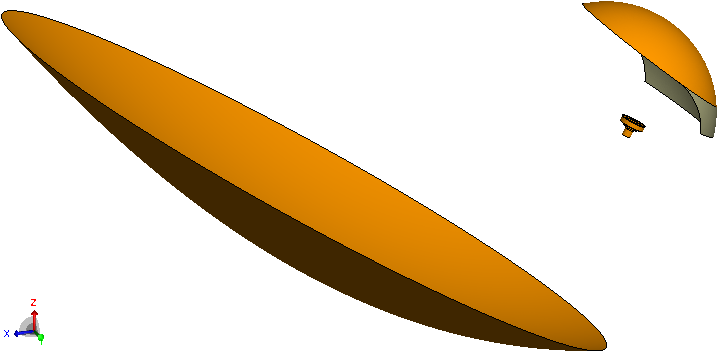
\includegraphics[width=258.48pt]{TU3e20-optics}
\caption{\label{fig:TU3e20:optics}The default offset Gregorian dish viewed from 
  $\theta=70^\circ$ (the angle from the optical axis which is here aligned with the 
  $z$-axis) and  $\phi=70^\circ$ ($20^\circ$ from full side-on).
  The sub-reflector extension is shown grey.}
\end{figure}

Generally the gain of dual reflector systems can be substantially improved by
shaping the optics.  This allows better use of the effective aperture leading to
higher gain, but typically also increased sidelobes.  With a -28~dB first
sidelobe specification, there is very little advantage in shaping the system.
The sidelobe specification is, however, done partly to improve imaging which is
the purpose of this comparison.  The specification was therefore relaxed to allow
testing the actual impact of the higher sidelobes.  The shaped option thus have
a -23~dB limit on the second sidelobe.  Shaped systems typically use a feed
horn with a narrower pattern as well as a larger sub-reflector edge angle.  This
results in a lower edge illumination and less lost spill-over efficiency.  (The
improved aperture illumination is achieved by spreading the feed pattern more
towards the edges of the main dish.)  Thus an additional feed horn was optimised
for this system.  As the shaped system already has less spill-over, the extension
on this design is only $15^\circ$ \citep{icea-dish-design}.  This is the shaped
OG option used here.

To really determine the impact of shaping, we also need to compare it with an
unshaped system having the same specifications.  (An unshaped system does allow
greater flexibility in the future, hence the shaped option should only be
considered if it is substantially better.) Hence a second feed was optimised for
the default OG dish with the relaxed sidelobe requirement.  This is the OG with
hard edge illumination used in this comparison.


\subsubsection{Calculated patterns}
\label{sec:patterns}

Fig.~\ref{fig:pb180} shows the full sphere normalised horizontal polarisation
beam patterns of the four optics candidates at 1440~MHz.  The patterns are
similar for vertical polarisation and also for all frequencies over the band
under consideration.  Fig.~\ref{fig:pb18} shows detail of the main beam region
of these patterns.

% The trim commands below remove the colourbar legends from the top images
\begin{figure*}
  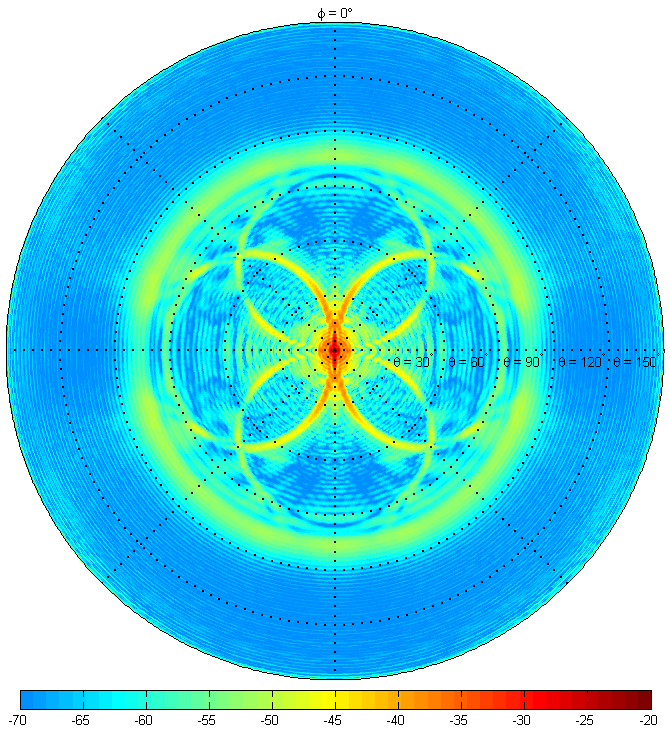
\includegraphics[width=\columnwidth,clip=true,trim=0 42 0 0]{K7s_full}\hfill%
  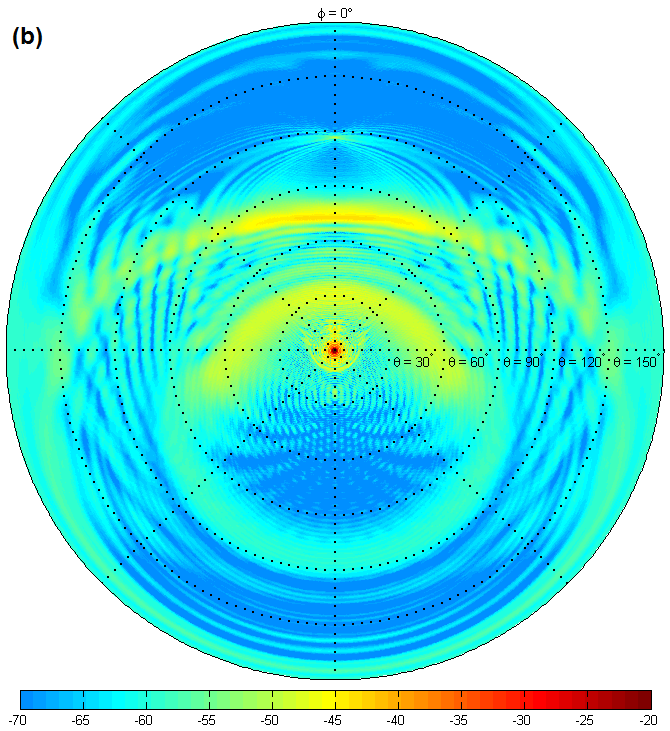
\includegraphics[width=\columnwidth,clip=true,trim=0 42 0 0]{TU3e20_full}
  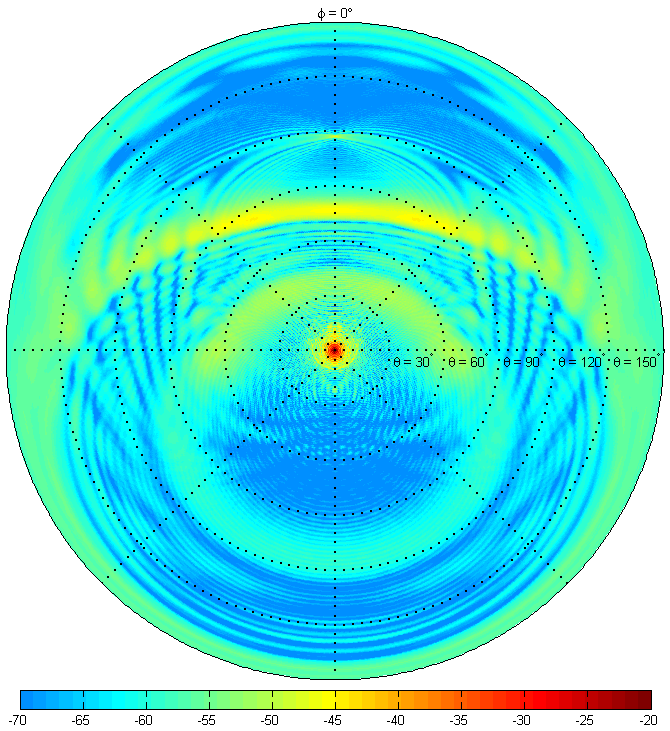
\includegraphics[width=\columnwidth]{TS3e15h_full}\hfill%
  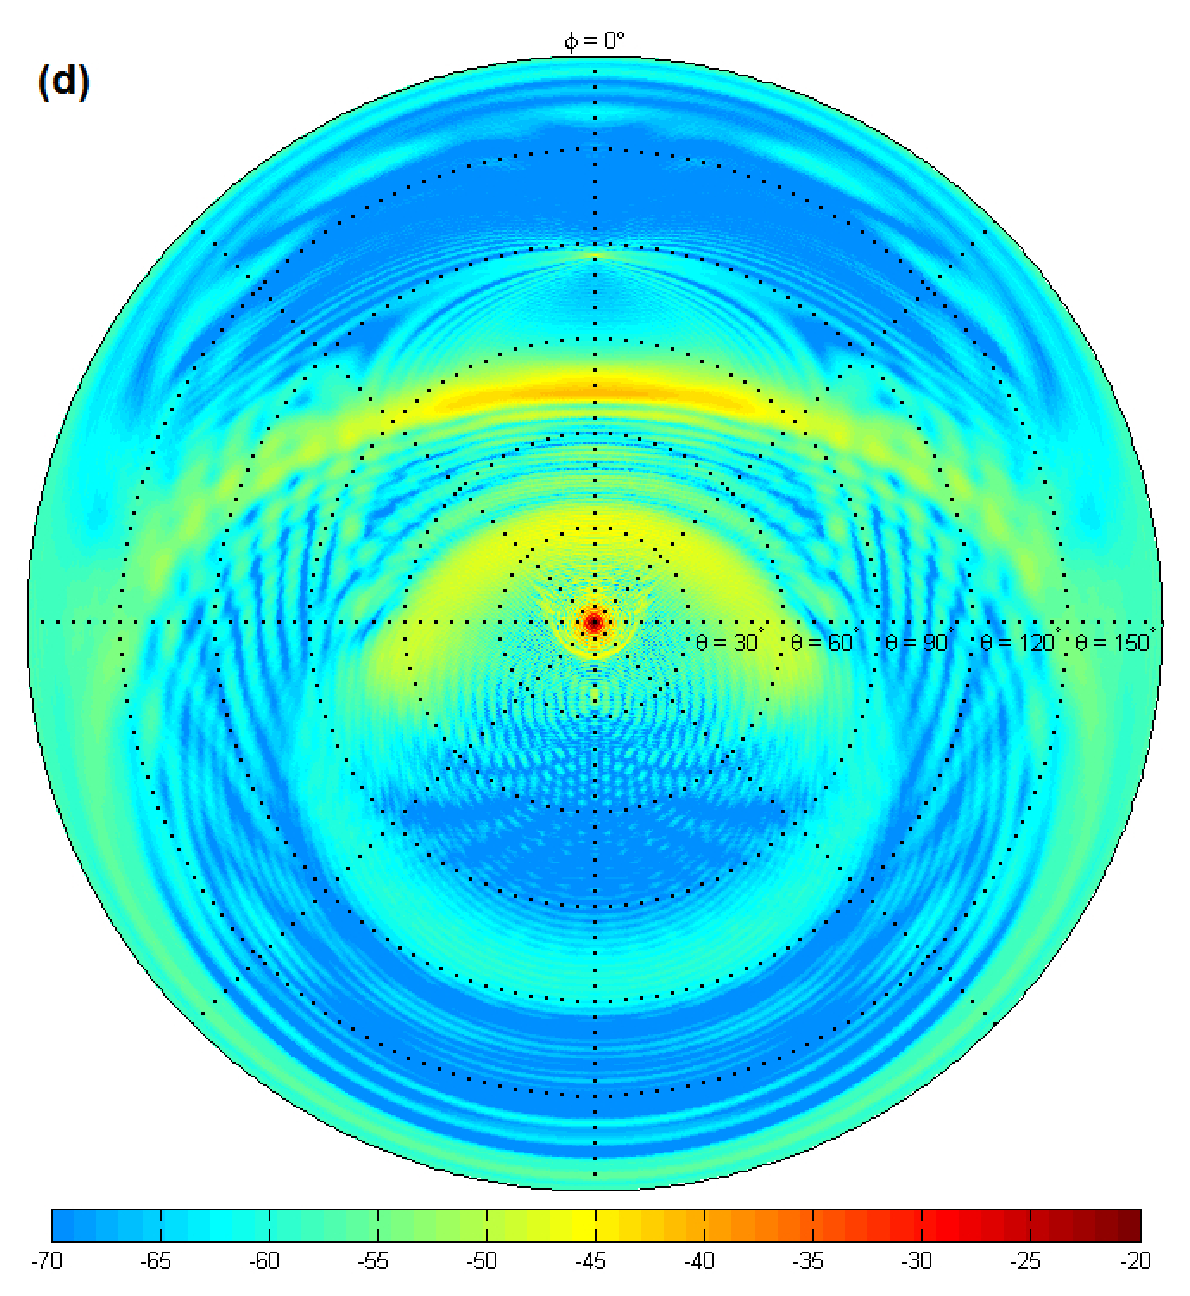
\includegraphics[width=\columnwidth]{TU3e20h_full}
  \caption{\label{fig:pb180}Normalised primary beam amplitude (in dB) for
    horizontal polarisation at 1440~MHz.  The pattern is displayed as a function
    of the polar coordinate angles $\theta$ (measured from the optical axis and
    displayed as the distance from the centre of these images) and $\phi$
    (measured around the $\theta=0^\circ$ axis and displayed on a constant
    radius in the figures).  The $\phi=0^\circ$ direction is vertical and upward
    if the alt-az mounted dish is pointing towards the horizon.  This
    "projection" opens the back half of the pattern outward -- the entire
    outside border (at $\theta=180^\circ$) corresponds to a single angular
    direction opposite the main beam. The top left picture (a) is for prime focus,
    the top right (b) for the default offset Gregorian; the bottom left (c) for the
    shaped offset Gregorian and the bottom right (d) for the offset Gregorian
    optimised with higher sidelobes (hard edge illumination).  For the offset
    Gregorian options, the projection of the sub-reflector is below these
    images, i.e.\ the main reflector lies towards $\phi=0^\circ$.}
\end{figure*}

\begin{figure*}
  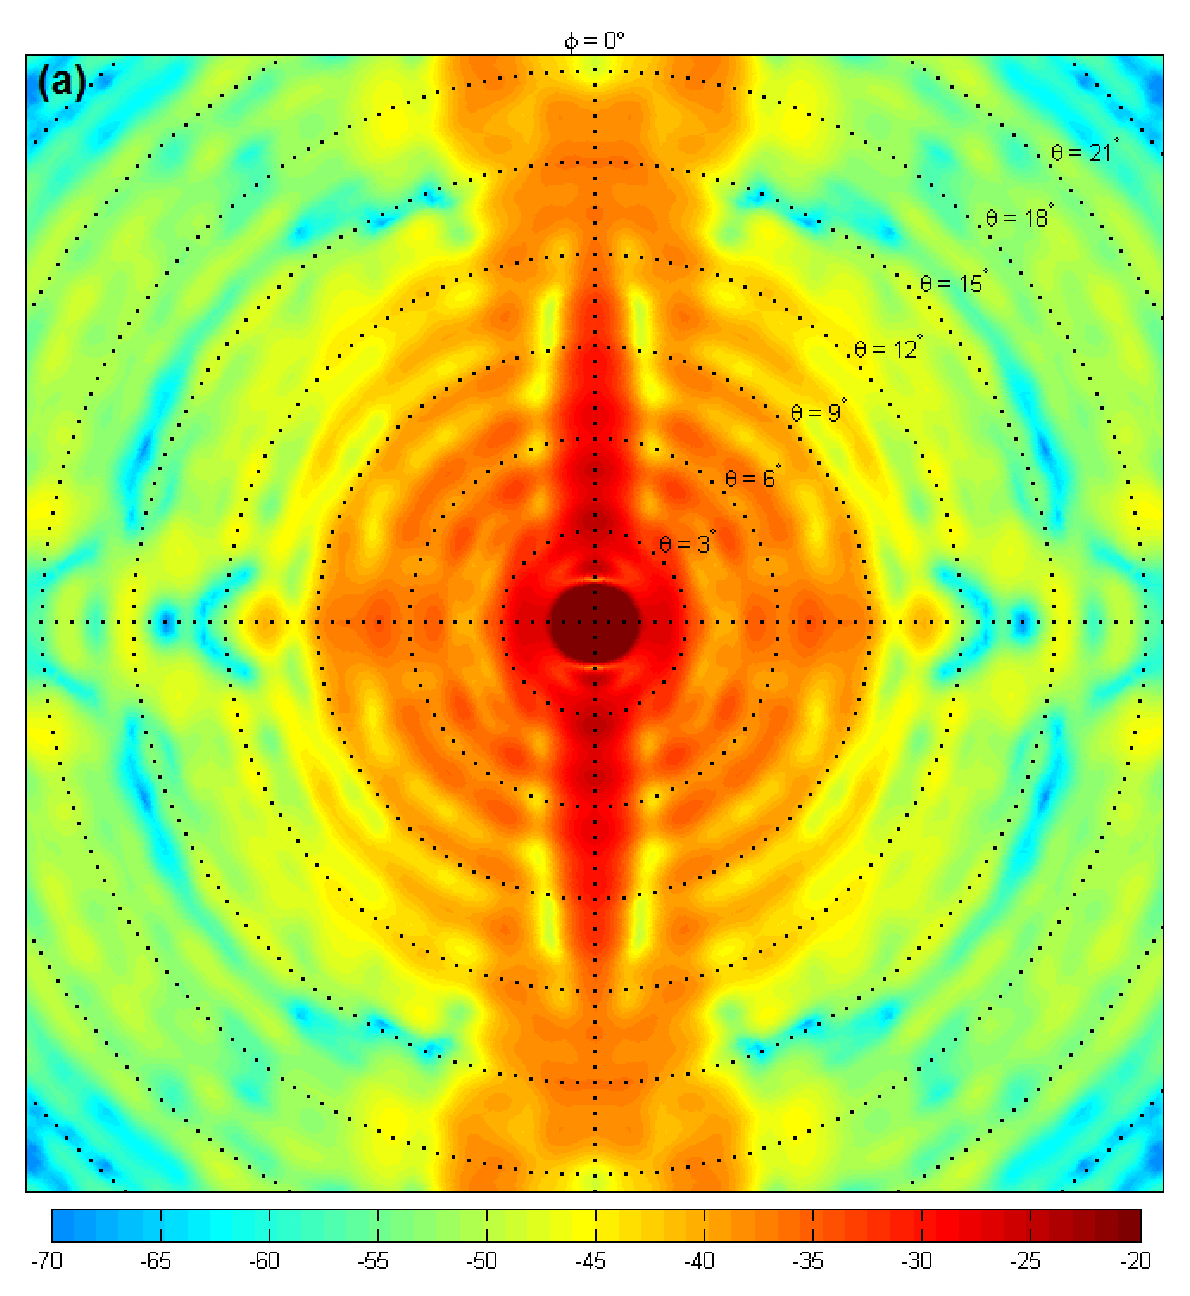
\includegraphics[width=\columnwidth,clip=true,trim=0 42 0 0]{K7s_main}\hfill%
  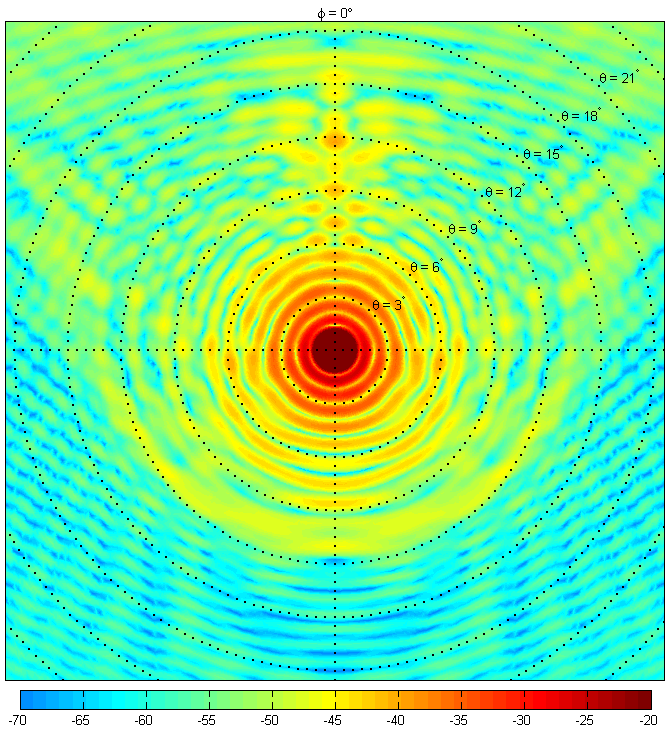
\includegraphics[width=\columnwidth,clip=true,trim=0 42 0 0]{TU3e20_main}
  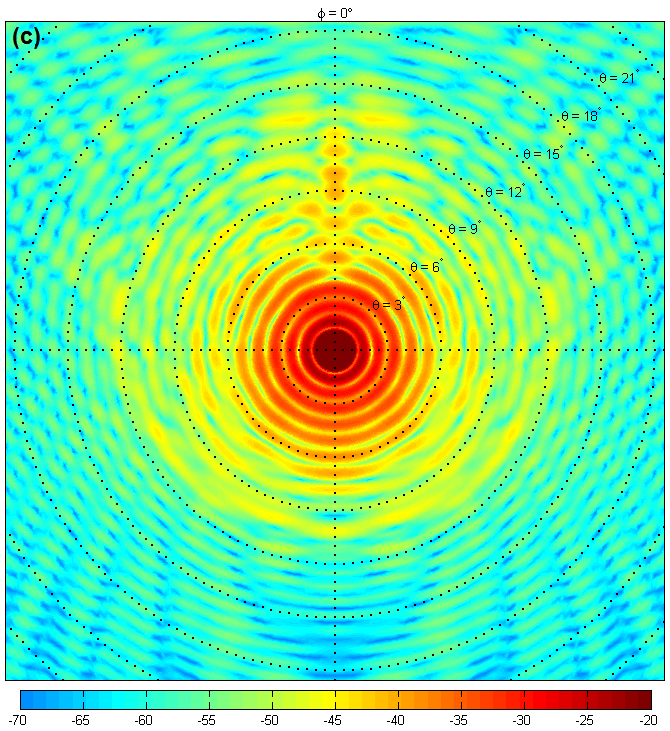
\includegraphics[width=\columnwidth]{TS3e15h_main}\hfill%
  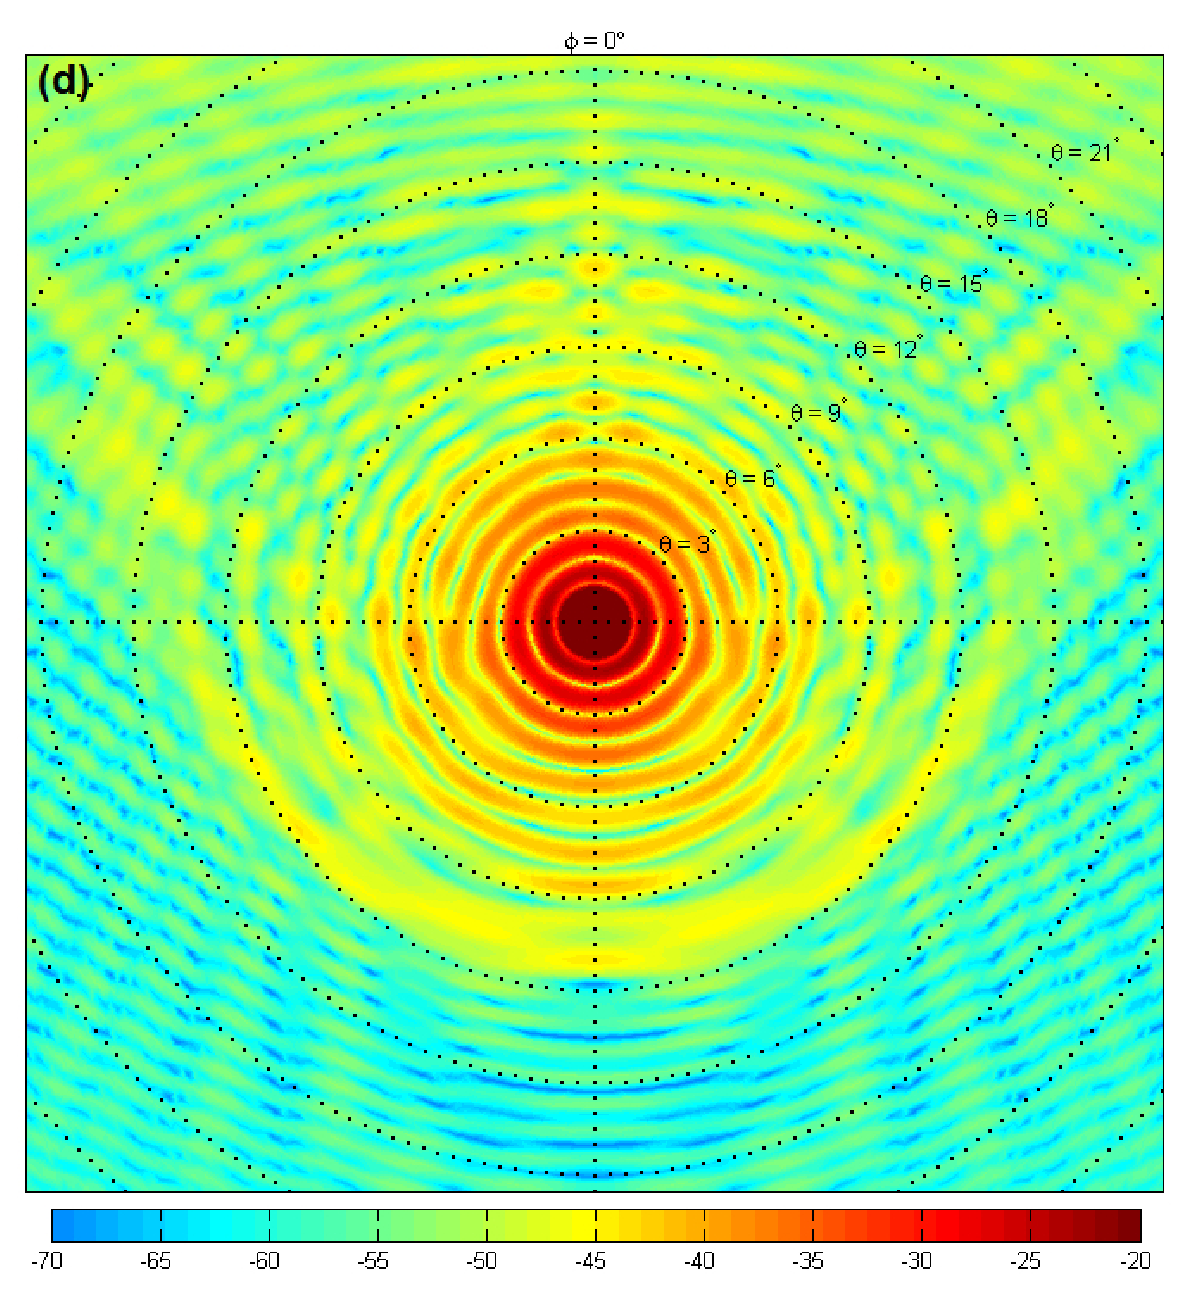
\includegraphics[width=\columnwidth]{TU3e20h_main}
  \caption{\label{fig:pb18}Primary beam amplitude (dB scale) for the main beam
    region of the patterns shown in Fig.~\ref{fig:pb180}.  The top left picture (a)
    is for prime focus, the top right (b) for the default offset Gregorian; the
    bottom left (c) for the shaped offset Gregorian and the bottom right (d) for the
    offset Gregorian optimised with higher sidelobes (hard edge illumination).}
\end{figure*}

For the prime focus dish, horizontal polarisation is blocked more by the
horizontal struts than the vertical ones such that the scattering cones
associated with the horizontal struts are larger than the other two.  This
results in a large "fan beam" sidelobe orthogonal to the polarisation direction
through the region of the main beam.  For vertical polarisation, it is the other
way around and the image is rotated by $90^\circ$.  The back lobes ($\theta >
90^\circ$) of the PF dish are primarily due to diffraction from the dish edge
with is at a constant distance from the feed.  Hence the back lobes are
relatively circular.

For the offset Gregorian patterns the first peak (roughly in the range $30^\circ
> \theta > 60^\circ$) is due to the spill-over from the feed past the
sub-reflector. This is markedly less for the shaped system due to its lower edge
taper.  In all OG cases, the sub-reflector extension ensure that this peak does
not close below the main beam (intercepting the ground as the dish is tipped
towards the ground).  The second peak (around $\theta = 75^\circ$ for $\phi =
0^\circ$) is due to the spill-over from the sub-reflector just above the main
reflector.  This line extends to $\theta = 180^\circ$ which is where the
spill-over from the sub-reflector passes the bottom of the main reflector.
These sidelobes are slightly lower in amplitude for the shaped system, but not
materially so.  The sharp peak at $\theta = 120^\circ$ and $\phi = 0^\circ$ is
the diffraction back lobe of the main reflector.

As expected the inner side-lobes for the shaped OG system and the hard edge
illuminated OG system are higher than for the default OG system.  Note also that
the general near-in sidelobes (in the absence of the strut scattering cones) of
the PF dish are indeed lower than for the OG system -- this is due to the
improved efficiency of all the OG systems.  The near-in sidelobes of the
unshaped OG systems appear a little more circular than for the shapes system,
but this is again not material.

It is interesting to note that the side-lobe spacing of the PF dish appears to
be double that of the OG dishes.  The reason for this is that alternating
side-lobes in the aperture pattern of the PF dish alternate in side and these
interfere constructively and destructively with the wide beam caused by the feed
blockage.


\subsection{Interferometric simulations}

The conventional approach to simulation in MeqTrees is to build a measurement
equation using the RIME formalism, and evaluate this equation for every time and
frequency bin of the desired MS. For an LSM consisting of a source catalog, a
typical RIME used in the present study would look as follows:

  \begin{equation}\label{eq:rime0}
  \coh{V}{pq} = \jones{G}{p} \left ( \sum_{s} S_{spq} {\jones{E}{sp} K_{sp} \coh{B}{s} K^\herm_{sq} \jonesT{E}{sq}} \right ) \jonesT{G}{q}
  \end{equation}

Here, $\coh{B}{s}$ is the brightness matrix of source $s$, $K_{sp}$ is the (scalar) phase term associated with station $p$  and direction $s$, $\jones{E}{sp}$ is the E-Jones, or primary beam gain term for station $p$ and direction $s$, $S_{spq}$ is a scalar smearing factor accounting for time and bandwidth averaging \citep[implemented as per Eq. (23) of ][]{RRIME1}, $\jones{G}{p}$ is the direction-independent gain term associated with station $p$, and $\jonesT{A}{}$ is the Hermitian (or conjugate) transpose of $\jones{A}{}$.

\subsubsection{Implementing a tensor RIME}

Recent developments in MeqTrees have been driven by the tensor RIME formalism suggested by \citet{RRIME4}. In particular, the inner sum over $s$ in Eq.~(\ref{eq:rime0}) can rewritten as an Einstein sum:

\begin{equation}
\label{eq:trime}
\tens{X}^{pi}_{qj} = 
  \tens{S}_{q}^{ps}\tens{E}_{s\alpha}^{pi}\tens{K}_{s}^{p}
  \tens{B}^\alpha_{\beta s}
  \bar\tens{K}_{q}^{s}
  \bar\tens{E}_{qj}^{s\beta}
\end{equation}

Mathematically, this is a straightforward equivalent of the sum in Eq.~(\ref{eq:rime0}), expressed in terms of a {\em brightness tensor} $\tens{B}^\alpha_{\beta s}$ of rank $N_s\times2\times2$, and a \emph{Jones tensor} of rank $N_p\times N_s\times2\times2$, where $N_p$ is the number of stations, and $N_s$ is the number of sources.

This form of the RIME has guided implementation of a new {\em tensor mode} framework in MeqTrees, which has led to a drastic reduction in {\em housekeeping overhead}. In MeqTrees, the housekeeping overhead of any given tree is the resource cost (in terms of CPU and RAM) associated with constructing and processing the basic computational units called {\em nodes}\footnote{That is, over and above the cost of the computations per se.}. Older versions of MeqTrees used $2\times2$ matrices as the basic computational unit, with a separate subtree per each station pair $pq$. Given a matrix RIME such as Eq.~(\ref{eq:rime0}), the housekeeping overhead of this approach scales as $O(N_p^2 N_s)$. Consequently, large-$N_p$ simulations (e.g. $N_p\gtrsim 30$) with MeqTrees were found to be dominated by housekeeping overhead rather than pure computational cost, with script compilations times and especially RAM usage becoming prohibitively high.

Tensor mode resolves this problem. The current implementation goes half-way to Eq.~(\ref{eq:trime}), in that the basic computational unit becomes the brightness tensor $\tens{B}$, and a \emph{per-station} Jones tensor $\tens{E}_p$, both of rank $N_s\times2\times2$. This has required the addition of only a single node class to MeqTrees, called {\tt PSVTensor} (``point source visibility tensor\footnote{Recent versions of {\tt PSVTensor} are making the name somewhat inaccurate, since they also include support for extended Gaussian components. The class will probably be renamed to {\tt DSVTensor} in the near future, with D standing for ``discrete''.}''), which implements Eq.~(\ref{eq:trime}) for a single $pq$ pair, given a brightness tensor, and any number of Jones tensors. Housekeeping costs then scale as the much more manageable $O(N_p^2+N_s)$. Note that the new tensor mode framework remains backwards-compatible with all the older MeqTrees Jones matrix modules, via the simple expedient of building up Jones 
tensors from $N_s$ separately generated Jones matrices. In this ``backwards compatibility'' regime the overhead scaling law is somewhat worse --  $O(N_p^2+N_p N_s)$ -- but this still better than the pure matrix regime. 

As an aside, we should note another advantage of using a tensor (rather than a $2\times2$ matrix) as the basic computational unit. The tensor approach explicitly groups related computations together into larger chunks, 
rather than spreading them through different nodes of the tree. This proves far more amenable to a GPU-based implementation. One result of this is the recent development of a {\tt CUDAPSVTensor} node class, which is 
essentially a CUDA-accelerated version of {\tt PSVTensor}. Since the two node classes are identical in terms of interface, MeqTrees is able to select at script complication time whether to use one or the other. This is still a work in progress -- in particular, {\tt CUDAPSVTensor} did not support E-Jones terms at time of writing, and so was not used to run the simulations reported on here -- but it shows great promise for the future.

%NB: need to update this with some performance figures once Richard's CUDA nodes work.

\subsubsection{Practical performance limitations}
\label{sec:performance}

In practical terms, tensor mode has allowed us to run simulations of a full MeerKAT layout ($N_p=64$) 
with $N_s=10^3\sim10^4$ discrete model sources, with full E-Jones treatment. To give some specific examples: the worst case scenario is a full per-station pointing error alt-az mount simulation (see below). This is completely dominated by evaluation of the E-Jones tensor, which then assumes a different value for each source, station and time/frequency bin. Such a simulation (for $\sim5000$ sources, 480 timeslots, 8 frequency channels) takes on the order of 10 hours on a modern 8-core machine without a GPU. For simulations without pointing errors, only a single E-Jones needs to be computed for all stations, and the same simulation runs to completion within an hour.

%NB: need to update this with some more accurate performance figures once Richard's CUDA nodes work.

\subsubsection{Partitioning the model sky}

Assuming $10^3\sim10^4$ discrete sources as a reasonable upper limit on a ``fast'' simulation, how deep a sky (in terms of limiting flux) can we accurately simulate? This of course depends how much sky area is being simulated. For example, given a $5\degr\times5\degr$ FoV, which at 1.4 GHz encompasses the main lobe and the first sidelobe of a MeerKAT primary beam, a full NVSS sampling (down to the limiting flux of 2.5 mJy) contains on the order of 1000 sources. On the other hand, for a full-sky FoV -- or more precisely a hemisphere (see simulations of Sect.~\ref{sec:fsn}) -- we get about 4000 sources at a cutoff flux of 0.5 Jy. 

Note that such limitations only apply to discrete models, in which every source gets the full individual E-Jones treatment of Eq.~(\ref{eq:rime0}) or Eq.~(\ref{eq:trime}). If we dispense with E-Jones (and all other direction-dependent Jones terms), then we can simulate a virtually unlimited number of fainter sources \emph{en masse}, by putting them into a sky image, applying an \emph{average} power beam to the image, and using an FFT to transform the image into predicted visibilities. There are at least three software tools that support\footnote{By which we also mean publicly available, and able to deal with measurement sets. The latter requirement rules out AIPS and other highly capable packages.}  this: the UVBrick component of MeqTrees \citep{Abdalla:uvbrick}, the CASA simulator tool, and the {\tt lwimager} tool. The latter has so far proven to be the most suitable, offering both a convenient single-command-line invocation (unlike CASA), and a full $w$-projection \citep{Cornwell:wproj} implementation (
unlike the UVBrick, for which $w$-projection it is still in development). 

An image-based simulation derived in this way cannot be entirely accurate, since it omits the E-Jones term (using at best a time- and station-average primary beam\footnote{The AW-projection algorithm \citep{SB:imageplane} does offer a way to incorporate virtually arbitrary DDEs into an FFT-based predict. However, currently available implementations do not yet support arbitrary E-Jones terms, and are therefore unsuitable for our purposes.}), and is also subject to pixellation errors. We therefore pick a flux threshold, and partition our sky models into two subsets:

\begin{itemize}
  \item A ``bright'' sky, which is simulated perfectly: that is, as a set of discrete sources with the full E-Jones treatment of Eq.~(\ref{eq:rime0}) or Eq.~(\ref{eq:trime}).
  \item A ``faint'' sky, which is simulated approximately: that is, as a single image attenuated by the average power beam $|\vec E|^2$. Presumably, this is faint enough for such an approximation to be sufficient.
\end{itemize}

The two subsets are simulated separately, and the resulting visibilities are simply added together.

For the limited-FoV simulations of Sect.~\ref{sec:dde}, it turns out to be most convenient to use the NVSS to provide a ``bright'' population of discrete sources from 3 mJy up, and S$^3$-SEX to provide a ``faint'' population from 3 mJy down. The latter was converted into a FITS image using the mapmaker script from the S$^3$-Tools package. 

For the full-sky simulations of Sect.~\ref{sec:fsn}, we dispensed with the faint sky altogether.

\subsection{Implementing E-Jones interpolation}

The RIME tells us how to apply an E-Jones to derive visibilities; determining the particular values that 
E-Jones assumes for every source and station is another matter entirely. The Cattery software framework included with MeqTrees provides a number of standard E-Jones implementations, in particular the
{\tt Cattery.Siamese.OMS.pybeams\_fits} module developed by one of the authors. This reads gridded complex beam patterns -- in other words, all four elements of the E-Jones matrix -- from FITS images. It then computes the position of each source in the local coordinate frame of the antenna (depending on whether sky rotation and/or pointing errors are included in the simulation, these positions may be time- and antenna-dependent), and interpolates the complex beam gains at that position from the gridded values. This module uses the MeqTrees pyNode extension, which allows nodes to be implemented in Python and embedded into computational trees alongside the native C++ node classes\footnote{The pyNode extension was originally intended for quick prototyping of new MeqTrees node classes (in ``slow'' Python), with the implicit understanding that the useful ones would be rewritten in ``fast'' C++ as needed. In practice, the emergence of the {\tt numpy} and {\tt scipy} libraries, which provide many useful -- and fast!
 -- array functions, has made it possible to write numerical code in Python that (in some cases) is almost as fast as compiled code. As a result, quite a few of our pyNode ``prototypes'', the {\tt pybeams\_fits} module being a prime example, have been quietly rebranded as production modules without any pressing need to be rewritten.}. Interpolation is done via the {\tt map\_coordinates} function found in the {\tt scipy} library. 

This implementation is quite generic, in the sense that arbitrary beam patterns may be provided as FITS files. However, since our EM simulations (Sect.~\ref{sec:emsims}) produce patterns in a spherical coordinate system, an intermediate regridding step is needed to convert these to FITS patterns suitable for use with {\tt pybeams\_fits}, which employ rectangular $l,m$ coordinates. We have therefore decided to implement a new E-Jones module based on this code, one that directly reads beam patterns gridded in spherical coordinates ($\theta,\phi$), and computes source positions and interpolates beam gains directly in the $\theta,\phi$ frame. The resulting E-Jones module is called {\tt emss\_beams}.

While developed for MeerKAT simulations, {\tt emss\_beams} is also quite generic, and could be used with any kind of primary beam, provided the beam patterns are gridded onto spherical coordinates, and written into a properly formatted ASCII file. It supports simultaneous interpolation through multiple superimposed patterns, with the resulting gains added together. This feature can be put to use in two particularly interesting ways. Firstly, the beam may be specified as a superposition of component patterns (e.g. main reflector, subreflector, feed). Secondly, different grid steps may be used for different parts of the beam, with e.g. a finer grid for the main lobe, and coarser grids for sidelobes. 

The variable grid step option is particularly important, since we need simulated beam patterns for the entire sky (or at least out to $\theta=90\degr$) on the one hand, and a high-resolution grid on the other (at least in the main lobe and first few sidelobes, where accuracy is important). The EM simulations of Sect.~\ref{sec:emsims} are extremely expensive computationally, so doing them for an entire hemisphere with a high-resolution grid would be prohibitively expensive. Instead, we separate the coordinate plane into six regions by $\theta$, i.e into an inner circle $0\leq\theta<\theta_1$, and 5 concentric annuli $\theta_{i-1}\leq\theta<\theta_i$, and use progressively coarser grid steps as we go out in $\theta$ (see Table~\ref{tab:grids}). 

\begin{table}
\begin{center}
  \begin{tabular}[]{ccccc}
  \hline
  \hline
  & & & &\\ [-1ex]
    region & $\theta$, from & $\theta$, to & $\Delta\theta$ & $\Delta\phi$ \\
  \hline
  & & & & \\ [-1ex]
    a & 0 & 0.25$\degr$ & 0.01$\degr$ & 2$\degr$ \\ 
    b & 0.25$\degr$ & 1$\degr$ & 0.025$\degr$ & 2$\degr$ \\ 
    c & 1$\degr$ & 4$\degr$ & 0.05$\degr$ & 2$\degr$ \\ 
    d & 4$\degr$ & 8$\degr$ & 0.1$\degr$ & 1$\degr$ \\ 
    e & 8$\degr$ & 30$\degr$ & 0.25$\degr$ & 1$\degr$ \\ 
    f & 30$\degr$ & 90$\degr$ & 1$\degr$ & 1$\degr$ \\ 
  \hline
  \end{tabular}
\end{center}
\caption{\label{tab:grids}Variable grid stepping in $\theta,\phi$ used for the beam pattern simulations.}
\end{table}


\subsubsection{Problems of complex interpolation} 

{\bf OMS: Discuss problems of interpolation -- a picture of the center ``nipple'' would be illuminating.}

\subsubsection{Interpolation in frequency.}

{\bf OMS: need to describe this.}


\section{Far sidelobe confusion noise (FSCN)}
\label{sec:fsn}

Sidelobe confusion, also called confusion noise, arises due to non-zero PSF sidelobe response away from centre. An interferometer does not sample the $uv$-plane fully, and gaps in the $uv$-coverage produce PSF sidelobes that are non-zero, even asymptotically. This in turn causes every source in the sky, no matter how distant, to contribute some ``confusing'' signal to every pixel of an interferometric map. Given a large number of sources, this contribution becomes essentially a random noise floor, thus justifying the name of confusion noise.

In practice, confusion noise is attenuated by a number of factors such PSF sidelobe level, primary beam sidelobe level and time/frequency averaging \citep[see Fig.~2 in][for an illustration]{SKA54-expa,SKA54}. Furthermore, by imaging and deconvolving sources within the FoV, one can progressively remove their contribution from confusion noise. This is what allows existing observatories to produce images that are limited by thermal noise (or calibration artefacts) rather than confusion. Typically, there's been little need to image and deconvolve sources beyond the main lobe, or at most the first sidelobe, of the primary beam, with sources in further primary beam sidelobes attenuated to negligible levels (barring pathological cases of really bright confusing sources in the sidelobes, which can be dealt with on an individual basis during calibration).

However, with the increased sensitivity of new instruments such as MeerKAT (and in the future the SKA), the thermal noise floor drops considerably. In particular, MeerKAT is designed to reach a thermal noise limit of 0.1 $\mu$Jy for a 5000-hour pointing. Such sensitivity levels make far-sidelobe confusion noise (FSCN) very much non-negligible. One would potentially need to image and deconvolve sources over a much larger sky area -- i.e. including the second, third, etc. primary beam sidelobe -- to reach the thermal noise again. This can potentially blow up computational costs, which scale directly with imaged sky area. The primary beam plays a crucial role in all this, since it attenuates the FSCN. As we show below, choice of optics can make an order of magnitude difference in FSCN levels.

\subsection{Prior work}

\citet[][see Appendix B]{VLA146} showed that FSCN can be analytically estimated as a random walk process in the complex plane. \citet[][]{SKA54-expa,SKA54} followed up on this in the context of SKA design. Distilling their results into a single equation (and using slightly different notation, for consistency with the present work), we have:

\newcommand{\DD}[1]{\,\mathrm{d}{#1}}

\begin{equation}
\label{eq:fscn}
  \sigma^2_\mathrm{FSCN}(r_0) = \left [ \int\limits_{r_0}^{\infty} P^2(r)C^2(r)E^2(r) \DD{r} \right ]
\left[ \int\limits_{0}^{S_\mathrm{max}} S^2n(S)\DD{S}\right ] 
\end{equation}

Here, $S$ is source flux, $n(S)$ is the differential source count, $P(r)$ is the PSF level at distance $r$ from centre, $C(r)$ is correlator attenuation due to time/bandwidth averaging, and $E(r)$ is the primary beam. However, as the individual terms in the first integration are difficult (if not impossible) to estimate analytically, this equation cannot easily be turned into quantitative estimates. Furthermore, it treats $P$ and $E$ as radially symmetric (although this can be generalized by using a two-dimensional integral). An even more subtle problem is that this formulation implicitly assumes a snapshot observation, and cannot properly account for time- and station-variable primary beams -- which can actually have quite a significant an impact on FSCN, as we'll show below.

The aim of this part of the work is therefore to use simulations to derive quantitative estimates of FSCN levels for different MeerKAT dish designs -- taking into account sky rotation and other effects -- and to establish a methodology for similar studies of SKA designs.

\subsection{Simulation technique}

The basic idea of a FSCN simulation is very simple. We take an all-sky model and make a hole in the middle: that is, exclude sources within a certain radius $r_0$ of the phase centre. Then, we run this model through an interferometric simulator with a variety of primary beam patterns, and use the resulting visibilities to make an image of the nominally empty sky in the middle. This image is non-zero due to FSCN, and the rms pixel value gives us the FSCN level corresponding to sources with $r>r_0$, i.e. the fundamental confusion noise floor that we can achieve by fully deconvolving an image of radius $r_0$.

Given the performance considerations of Sect.~\ref{sec:performance}, complete and sufficiently deep all-sky simulations are impractical due to the very high source counts. We have therefore taken a few shortcuts:

\begin{itemize}
  \item We only simulate a hemisphere (i.e. to a radius of $90\degr$ from phase centre) and not the full sky, and we do not take into account horizon masking. As we shall see later, the bulk of FSCN is contributed by sources within $10\degr$ of centre, so this shortcut is justified. A proper analysis of the effects of this shortcut is given in Sect.~\ref{sec:horizon-masking}.
  \item We restrict each simulation to $\sim4000$ sources at a time; we have therefore imposed a lower flux threshold of 0.5 Jy, and extrapolate the contribution of fainter sources as discussed in Sect.~\ref{sec:source-counts}.
  \item To reduce data size, we typically simulate only a few frequency channels, and use relatively long (60~s) integrations. The effect of this on our FSCN results is discussed further in Sect.~\ref{sec:smearing}.
\end{itemize}

\subsection{Observational configuration}
\label{sec:config}

The observational configuration used in the simulation is set up by generating an ``empty'' measurement set with appropriate metadata, for which we use the {\tt makems} tool\footnote{{\tt makems} is standalone utility written by Ger van Diepen which generates measurement sets based on simple configuration files. It is available from the MeqTrees (and LOFAR) software repositories. The simulation tools found in CASA may also be used for this purpose.}. For the FSCN simulations, we have used the following configuration: 64-dish MeerKAT layout (cite?), 8 hour observation, field centred at RA=0h, Dec=-40\degr, 60~s integration, 8 channels, 20~MHz band centred on 1450~MHz. We shall refer to this as the ``canonical'' configuration from now on.

A real-life MeerKAT observation would use shorter ($\leq10$~s) integrations, and a much wider band, with more frequency channels. This does have an impact on FSCN levels, but not a major one. Sect.~\ref{sec:smearing} examines this issue in more detail.

\subsection{Sky models}

To make the sky models for this simulation, we extracted NVSS samplings of complete hemispheres, with a lower flux cutoff of 0.5~Jy. This resulted in roughly 4000 sources per hemisphere, depending on choice of centre (Fig.~\ref{fig:ncp-skymodel}). To simplify processing, each hemisphere was then shifted to the nominal phase centre of our simulated observation (RA=0h, Dec=-40\degr), using the Tigger sky model management tool included with MeqTrees.

\begin{figure}
\centering 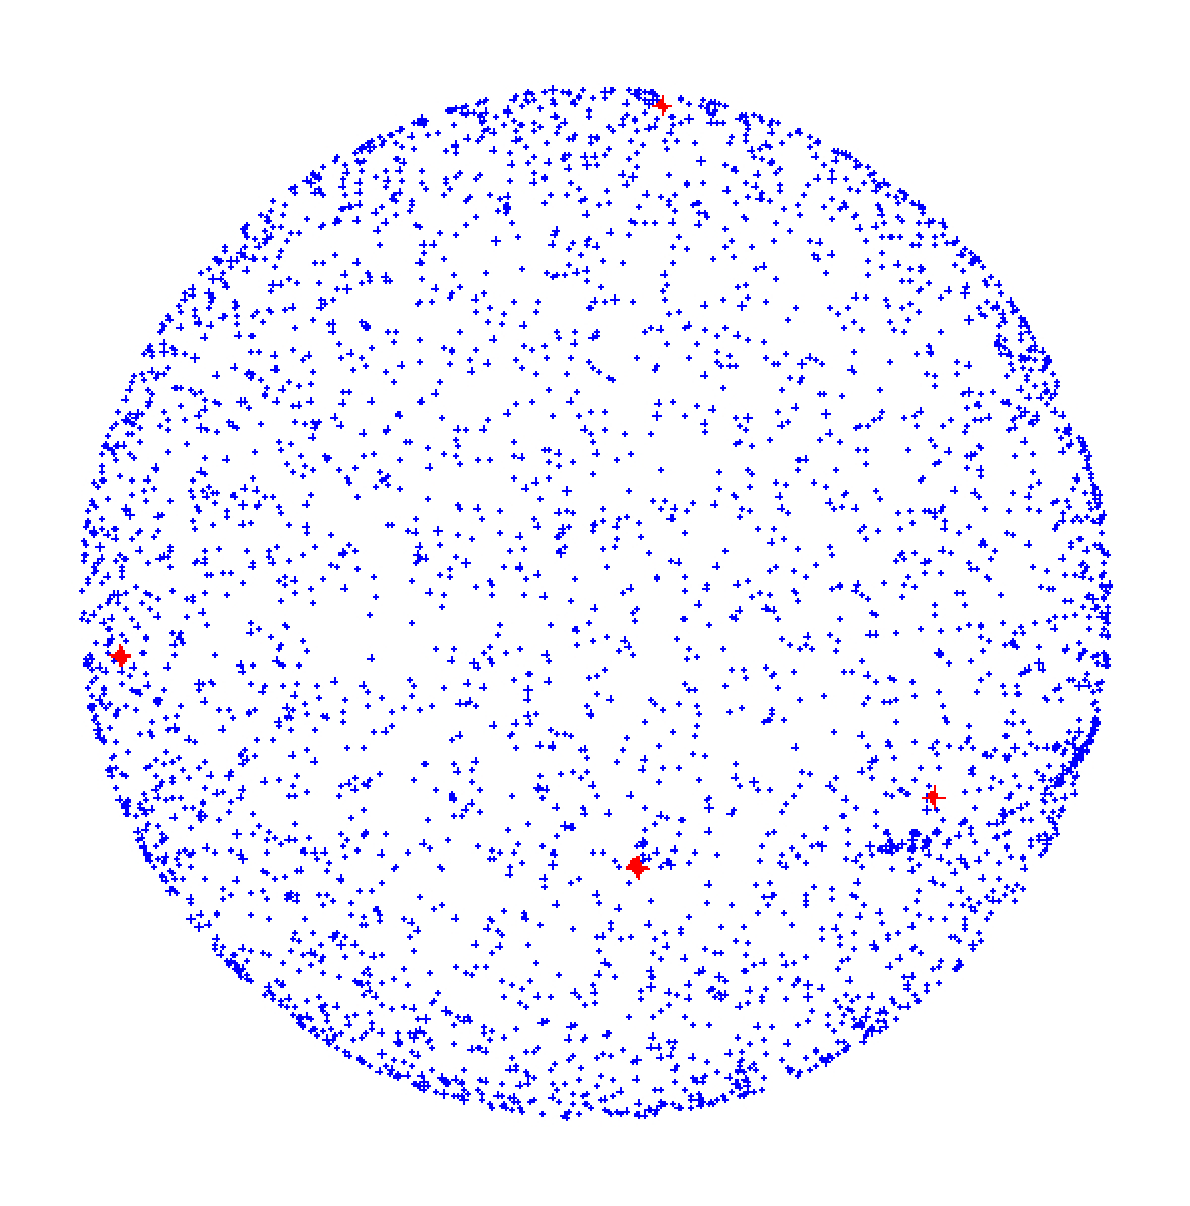
\includegraphics[width=.7\columnwidth]{ncp-skymodel-transp}
\caption{\label{fig:ncp-skymodel}A typical hemisphere sky model used for the FSCN simulation. This particular hemisphere was centred on the NCP, i.e. this is essentially just the Northern sky between 0.5 and 3 Jy. Source clusters associated with the A-team are indicated in red.}
\end{figure}

\begin{figure*}
  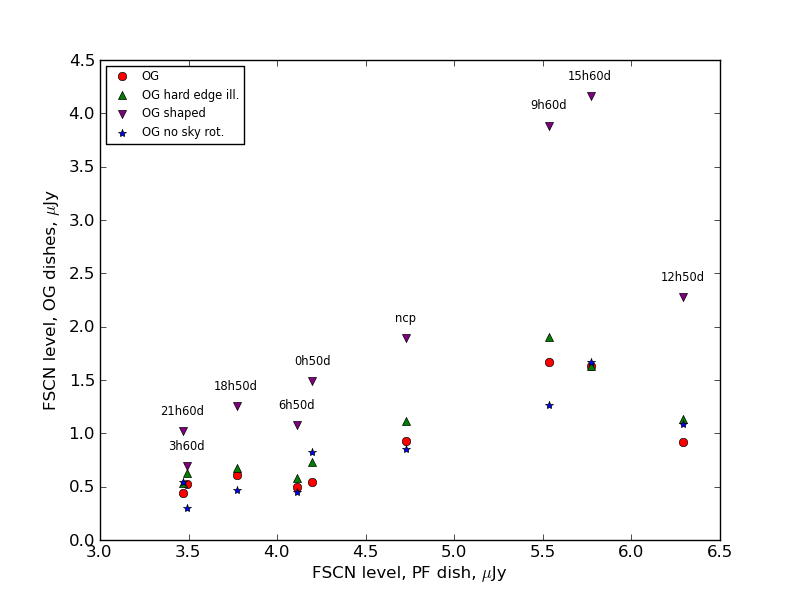
\includegraphics[width=\columnwidth]{cc-fields-325}
  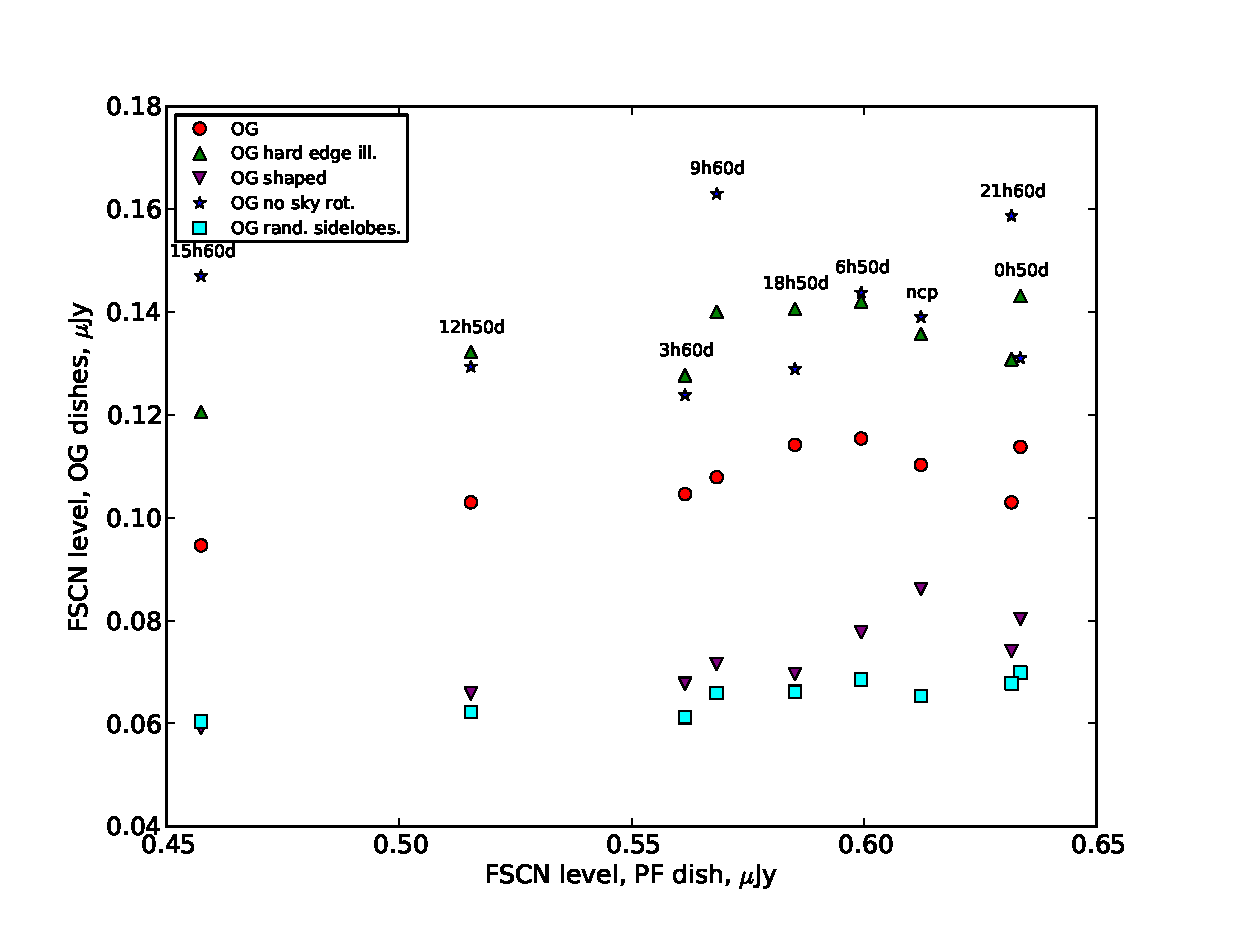
\includegraphics[width=\columnwidth]{cc-fields-10}
%  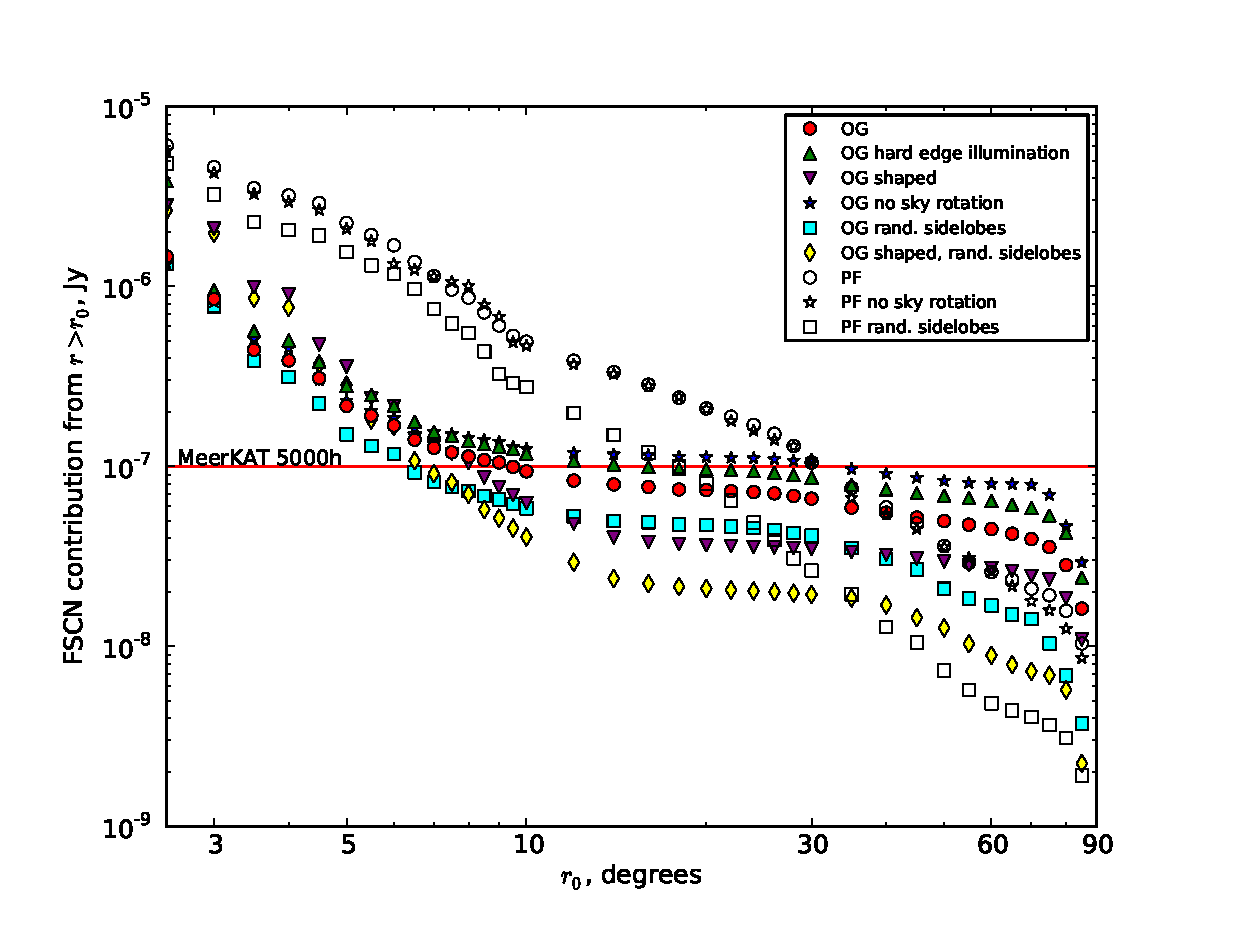
\includegraphics[width=\textwidth]{costcurve-main}
\caption{\label{fig:fscn-fields}FSCN levels (offset Gregorian vs. prime focus) for the 9 hemisphere models used in the simulations. The plot on the left is for $r_0=3.25\degr$, the plot on the right is for $r_0=10\degr$. The increased variance in the left plot is caused by the stronger close-in sidelobes. Note how the shaped OG design is especially susceptible to this.}
\end{figure*}

A handful of the strongest sources in the sky -- the ``A-team'' of  Cas~A, Vir~A, etc. -- can provide a dominant contribution to FSCN even from relatively distant sidelobes. This is a well-known problem, and current real-life data reduction practice is to treat such sources on an individual basis, by including them in the calibration model. Their contribution is thus effectively removed even before imaging. We have therefore excluded the A-team -- or, more generally, all sources brighter than 3~Jy -- from the sky models, on the assumption that such sources would have to be subtracted individually during calibration anyway. We also found that a simple 3~Jy cutoff was insufficient, as the NVSS represents each A-team source by a whole cluster of point sources, with a large number of them slipping below the threshold of them 3~Jy, but making a noticeable FSCN contribution through sheer numbers. We therefore removed such clusters from the models by hand.

We also noticed early on that even with the A-team excluded, our simulations were still fairly sensitive (at least for smaller values of $r_0$) to choice of sky model, which is probably due to small number statistics, i.e. a dominant contribution from a few of the brighter close-in sources sitting in (or passing through) particularly strong sidelobes. Figure~\ref{fig:fscn-fields} provides an indication of how FSCN varies across the 9 hemisphere models. This plots the simulated FSCN corresponding to the various offset Gregorian flavours against that for the prime focus dish, for all 9 models. The plot on the left is for $r_0=3.25\degr$ (third sidelobe and out), the plot on the right is for $r_0=10\degr$. It is clear that most of the variation is caused by the close-in sidelobes: there's roughly a factor of 2 variation across models at $r_0=3.25\degr$ (even more than 2 for the shaped OG design, which is to be expected, given it's higher close-in sidelobes), but considerably less than that at $r_0=10\degr$. In 
order to reduce this variance, we average FSCN levels (quadratically, since this is rms) across all 9 fields in all subsequent plots.

\subsection{Source counts and extrapolation to fainter sources}
\label{sec:source-counts}
% 304,538,103 sources in the Wilman sim.

The FSCN value described by Eq.~(\ref{eq:fscn}) includes a term which depends on the integral of the differential source counts $n(S)$. Since our measured values of FSCN are derived from simulations using a sky model with source fluxes in the range 0.5~$\leq$~$S$~$\leq$~3 Jy they are missing a potentially significant contribution from the faint source population. In this section we derive a correction factor to the FSCN values of the form

\begin{equation}
\left[\frac{\sigma_{0}}{\sigma_{0.5}}\right]^{2} = \left[\int\limits_{0}^{S_\mathrm{max}} S^{2}~n(S)~dS\right]  \left[\int\limits_{0.5}^{S_\mathrm{max}} S^{2}~n(S)~dS\right]^{-1},
\label{eq:fscn_correction}
\end{equation}

\noindent where $\sigma_{0}$ is the \emph{true} FSCN value including all sources up to a flux limit $S_\mathrm{max}$, and $\sigma_{0.5}$ is the FSCN level including only the sources between our lower flux cut off of 0.5~Jy and $S_\mathrm{max}$. Note that $S_\mathrm{max}$ is set to 3 Jy when evaluating the integrals due to the 3~Jy upper flux limit imposed to exclude the A-team sources. 

As is consistent with the sky model setup described in Section 2.1, the integrated source counts for the correction factor are computed from the S$^{3}$-SEX simulation \citep{Wilman-simulation}. The 1.4~GHz flux densities of the $\sim$300 million sources in the simulation are first placed into 250 logarithmically spaced flux bins, forming $n(S)$ and allowing Eq.~(\ref{eq:fscn_correction}) to be numerically evaluated, resulting in a value of $\sigma_{0}$/$\sigma_{0.5}$~=~3.66.

The differential source counts derived from the Wilman simulation are shown by the black squares on Fig.~\ref{fig:source_counts}. The distribution is Euclidean-normalized for ease of comparison to observationally-derived values which are shown by the red circles. Details of these data and an review of the subject of radio source counts are provided by \citet{deZotti-surveys}. 

The limitations of the S$^{3}$-SEX simulation are described by \citet{Wilman-simulation}, but of particular concern for this work is the possible significant deviation of the simulation from the observed source counts at sub-mJy levels, and the implications this may have for the correction factor described by Eq.~(\ref{eq:fscn_correction}). The observations in Fig.~\ref{fig:source_counts} show a flattening, or possible turn-up in the source counts at the faint end of the distribution. This picture is reinforced by the triangles on Fig.~\ref{fig:source_counts} which are the radio source counts derived by applying infrared-radio correlations to the $K$-band luminosity function, which has been explored down to very faint levels (Jarvis 2012, in prep.). The completeness limit of the $K$-band data causes the sudden decline which does not reflect the true behaviour of the counts.

The observed inflection in the source counts remains the subject of much debate and is generally thought to be caused by the dominant source population shifting from active galactic nuclei (AGN) to star-forming galaxies at these flux levels \citep[e.g.][]{Padovani-VLA-Chandra-DFS} although radio-weak AGN may also be a significant contributor to the counts \citep{Simpson-Subaru-XMM}. 

For reasons of consistency we adopt the previously derived value of 3.66 for the FSCN correction factor in the simulations that follow. However given the deviation of the simulation from the observations which we have outlined above, and in order to probe how much we may be underestimating the FSCN correction factor, we also implement a toy model which deviates from the S$^{3}$-SEX simulation at the approximate point where the counts begin to turn up, as marked by the dashed vertical line on Fig.~\ref{fig:source_counts}. This model is implemented by applying a power-law correction to the S$^{3}$-SEX counts which is unity at the marked cross-over point and increases with decreasing flux such that the new model approximately tracks the upper envelope of the observed values. This model is shown on Fig.~\ref{fig:source_counts} by the small black dots. 

Evaluating the correction factor for the toy ``extreme faint counts" model results in value of 6.72, a factor $\simeq$1.8 higher than the adopted value. This demonstrates that the ``cost curves" we derive in the following section are not critically sensitive to the size of the unknown faint source population, even for unrealistically large counts.

Future deep surveys with new and improved radio interferometers such as the EVLA and MeerKAT \citep[e.g.][]{Jarvis-MeerKAT-SALT,Heywood-MESMER} will probe the extremely faint end of the source count distribution. Such experiments form one of the many reasons why the investigation of hitherto negligible effects such as FSCN is vital.

\begin{figure}
\centering
%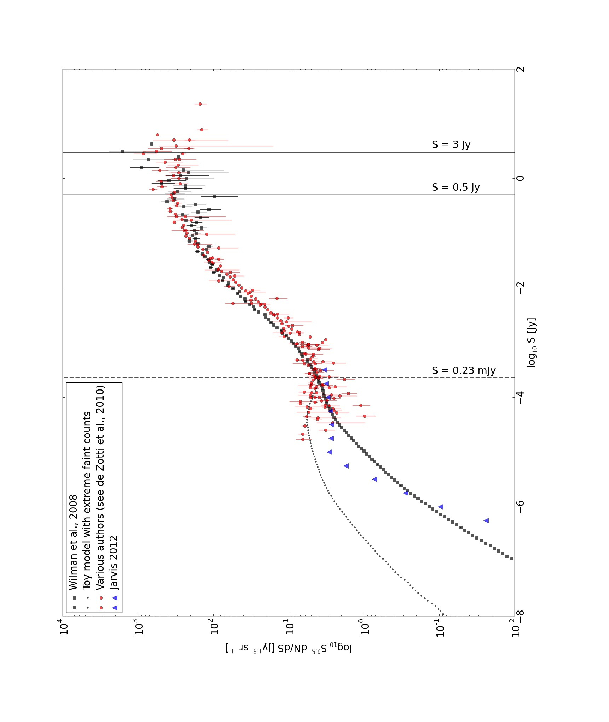
\includegraphics[width = 0.8 \textwidth]{1400_source_counts}
\caption{Euclidean-normalised radio source counts at 1.4 GHz. The red data points represent counts derived by several authors, as collated by \citet{deZotti-surveys}. The black squares show the source counts from the S$^{3}$-SEX simulation derived by binning all $\sim$300 million sources over the full 400 square degree sky area into 250 logarithmically-spaced flux bins. The triangles are radio source counts derived from $K$-band infrared magnitudes (Jarvis 2012, in prep.). The two solid vertical lines span the flux density range over which NVSS sources are selected. The small black squares show the toy model which we implement to investigate the potential effect of an extremely large population of faint sources. The model applies a power-law modification to the S$^{3}$-SEX counts and the point where the models converge is marked by the dashed vertical line.  \label{fig:source_counts}}
\end{figure}

\subsection{The classical confusion limit}

An image of the sky reaches the classical confusion limit when the background source population can no longer be resolved into individual sources, i.e.~when the density of sources $n(S)$ reaches a critical value. Depending on the spatial resolution of the instrument the confusion limit places a fundamental limit on the depth that can be reached by any observation.

In this section we compute the confusion limit of MeerKAT. The area of the PSF ($\Omega_\mathrm{PSF}$) for MeerKAT is determined by running a full 12-hour synthesis simulation ($\nu_\mathrm{min}$~=~1.440 GHz, $\Delta \nu$~=~20~MHz) for a variety of Declinations: 0$^{\circ}$, -30$^{\circ}$, -60$^{\circ}$ and -90$^{\circ}$. A 2D Gaussian is then fitted to the main lobe of the PSFs derived from these simulations for both uniform and natural weighting of the visibilities. The PSF parameters are given in Tab.~\ref{tab:conf_beams}.

The density of sources within a PSF area is determined by using the source counts from the S$^{3}$-SEX simulation \citep{Wilman-simulation}. For a given RMS noise value $\sigma_\mathrm{map}$ the number of detected sources per square degree is calculated: $n(S > \sigma_\mathrm{map})$. There is no formal definition for the number of PSF areas per source below which the map is said to be confusion limited, so we adopt the often-used rule-of-thumb which places the number at 10. The map is thus confusion limited if the following condition is satisfied:

\begin{equation}
n(S > \sigma_\mathrm{map})~\Omega_\mathrm{PSF} > 1 / 10.
\label{eq:conf_limit}
\end{equation}

Four Declinations and two weighting schemes means that we calculate the confusion noise $\sigma_\mathrm{conf}$ for eight different scenarios. The source count data described in Sect.~\ref{sec:source-counts} is employed here, with the confusion limit determined by the lower edge of the flux bin in which the condition in Eq.~(\ref{eq:conf_limit}) becomes satisfied for each of the eight beam sizes. The beam sizes and the results are given in Tab.~\ref{tab:conf_beams} and the confusion limit is shown graphically in Fig.~\ref{fig:conf_limits}. The actual quoted flux limits are subject to an uncertainty associated with the width of the bin, which is $\sim$10\% at these levels. The density of sources $n(S)$ is also averaged over the full sky area of the simulation, whereas in reality this will be dependent on the clustering strength due to cosmic variance. For comparison, the L-band confusion limit of the Very Large Array in D-configuration\footnote{{\tt http://www.vla.nrao.edu/astro/guides/vlas/current/node11.html}
} (
maximum baseline = 1~km) is 86~$\mu$Jy beam$^{-1}$.

\begin{table*}
\centering
%\begin{minipage}{158mm}
\caption{Uniform and naturally weighted PSF properties for the MeerKAT array at 1.4 GHz for a variety of Declinations, and the corresponding approximate confusion noise limit.\label{tab:conf_beams}}
\begin{tabular}{llllll}
\hline
\hline
Declination (deg) & Weighting scheme & $B_{maj}$ (arcsec) & $B_{min}$ (arcsec) & PA (deg) & $\sigma_{conf}$ ($\mu$Jy beam$^{-1}$) \\ \hline
0   & natural & 15.18 & 12.85 & -12.98 & 156\\
-30 & natural & 13.94 & 12.78 & 107.00 & 139\\
-60 & natural & 13.85 & 12.45 & 96.70  & 139\\
-90 & natural & 13.90 & 13.87 & 30.53  & 156\\
0   & uniform & 6.94  & 6.48  & -28.55 & 41\\
-30 & uniform & 5.66  & 5.33  & -51.08 & 30\\
-60 & uniform & 5.40  & 5.12  & 115.84 & 26\\
-90 & uniform & 5.27  & 5.26  & 52.03  & 26\\ \hline
\end{tabular}
%\end{minipage}
\end{table*}

\begin{figure}
\centering
%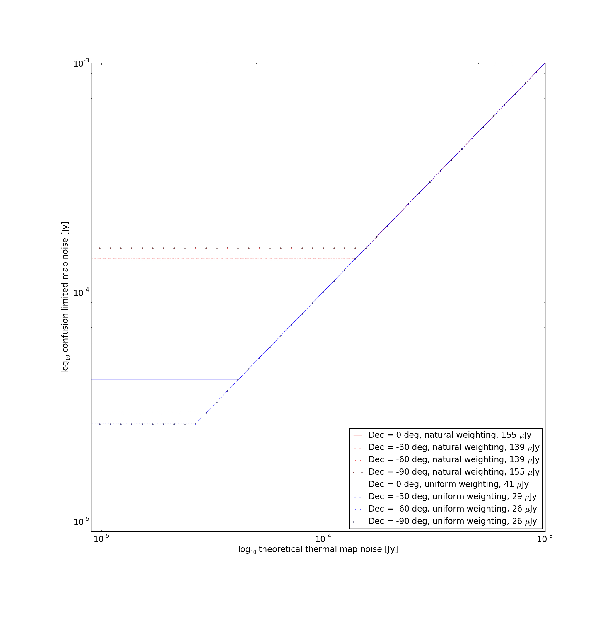
\includegraphics[width = 0.8 \textwidth]{1400_confusion}
\caption{The effects of the classical confusion limit on a 1.4 GHz MeerKAT observation. The abscissa represents the theoretical map noise as derived by the standard noise equation for a radio interferometer. The ordinate shows the corresponding classical confusion noise limit for a map that reaches a particular depth. The beam areas are calculated from a full 12-hour synthesis for four Declination values, and for both uniform and naturally weighted images.\label{fig:conf_limits}}
\end{figure}

% Having imposed a lower flux cut-off of 0.5 Jy for practical reasons, we end up missing an extremely significant contribution from the massive population of weaker sources. In terms of Eq.~(\ref{eq:fscn}), our simulations correspond to limits of $0.5$ to $S_\mathrm{max}=3$ on the second integral (rather than $0$ to $3$). From this it follows that the factor by which we underestimate the FSCN in our simulations is
% 
% \begin{equation}
% \left [ \frac{\sigma_\mathrm{0}}{\sigma_\mathrm{0.5}}\right ]^2 = 
% \left [ \int\limits_{0}^{S_\mathrm{max}} S^2n(S)\DD{S} \right ] 
% \left [ \int\limits_{0.5}^{S_\mathrm{max}} S^2n(S)\DD{S} \right ]^{-1},
% \end{equation}
% 
% where $\sigma_0$ is the ``true'' FSCN level corresponding to the entire source population, and $\sigma_{0.5}$ is the FSCN contribution from sources brighter than $0.5$ Jy.
% 
% {\bf OMS: Ian, this is your section. Please use Wilman's raw numbers for $n(S)$ to evaluate the equation above and derive a correction factor. A pretty plot of $S^2n(S)$ versus $S$ would also be illuminating.}
% 
% {\bf As a quick-and-dirty ``empirical'' check, what I've done so far is taken a deep S3-SEX query, built a cumulative histogram of $S^2n(S)$, and numerically integrated from 0 to $S_{max}$=3 and from 0.5 to 3. This gave me a ratio of about 7$\sim$10 between the two integrals, so I've been conservatively using $\sqrt{10}$ as the correction factor thus far.}
% 
% The resulting correction factor of $\sqrt{10}$ has been applied to all simulation results below. 



\subsection{MeerKAT results}
\label{sec:meerkat-costcurve}

\begin{figure*}
  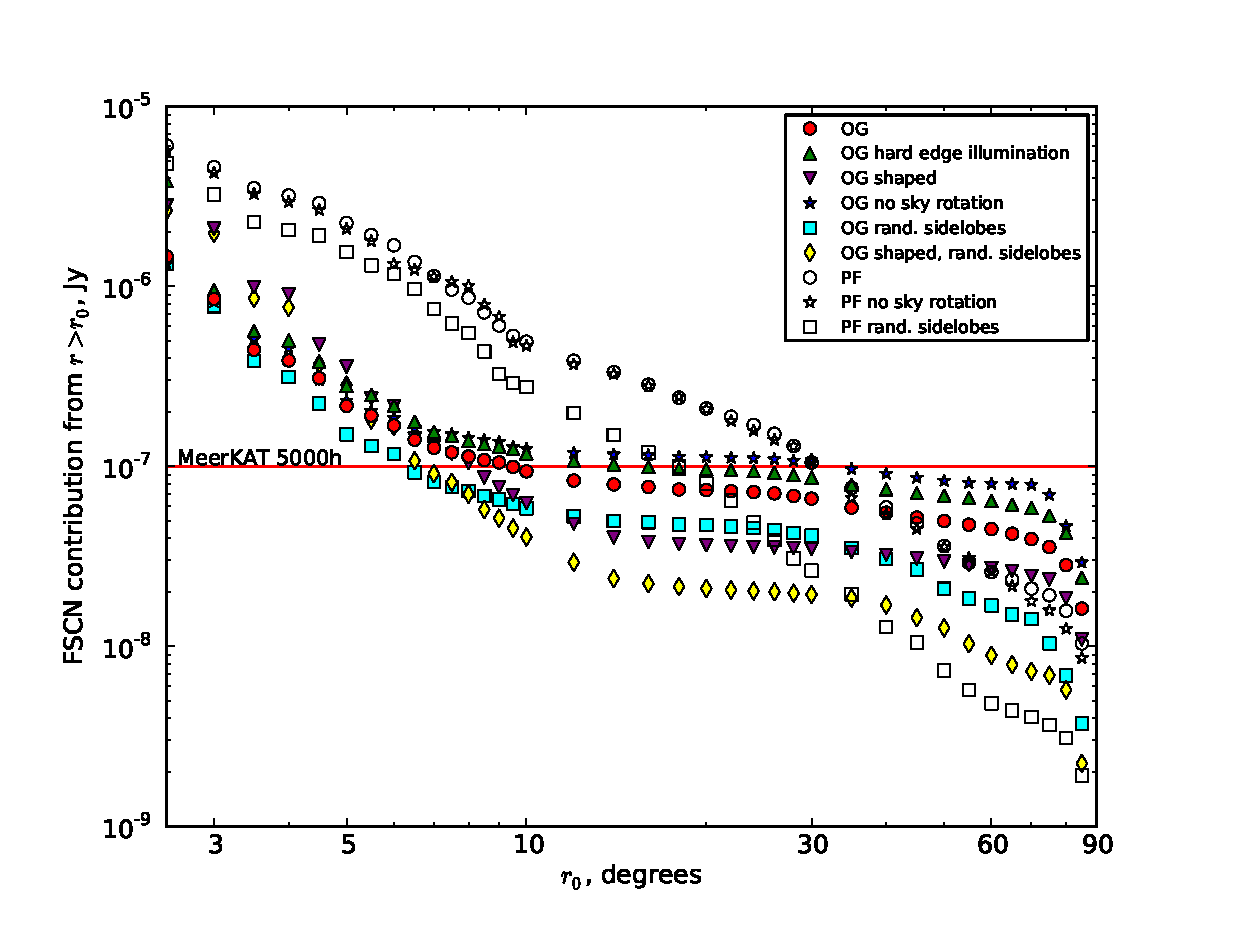
\includegraphics[width=\textwidth]{costcurve-main}\hfill
%  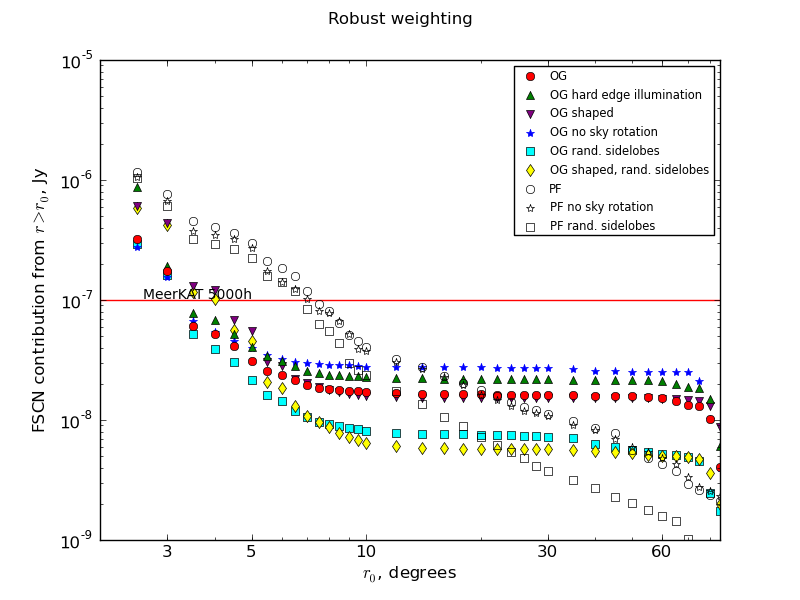
\includegraphics[width=\columnwidth]{costcurve-main-robust}
%  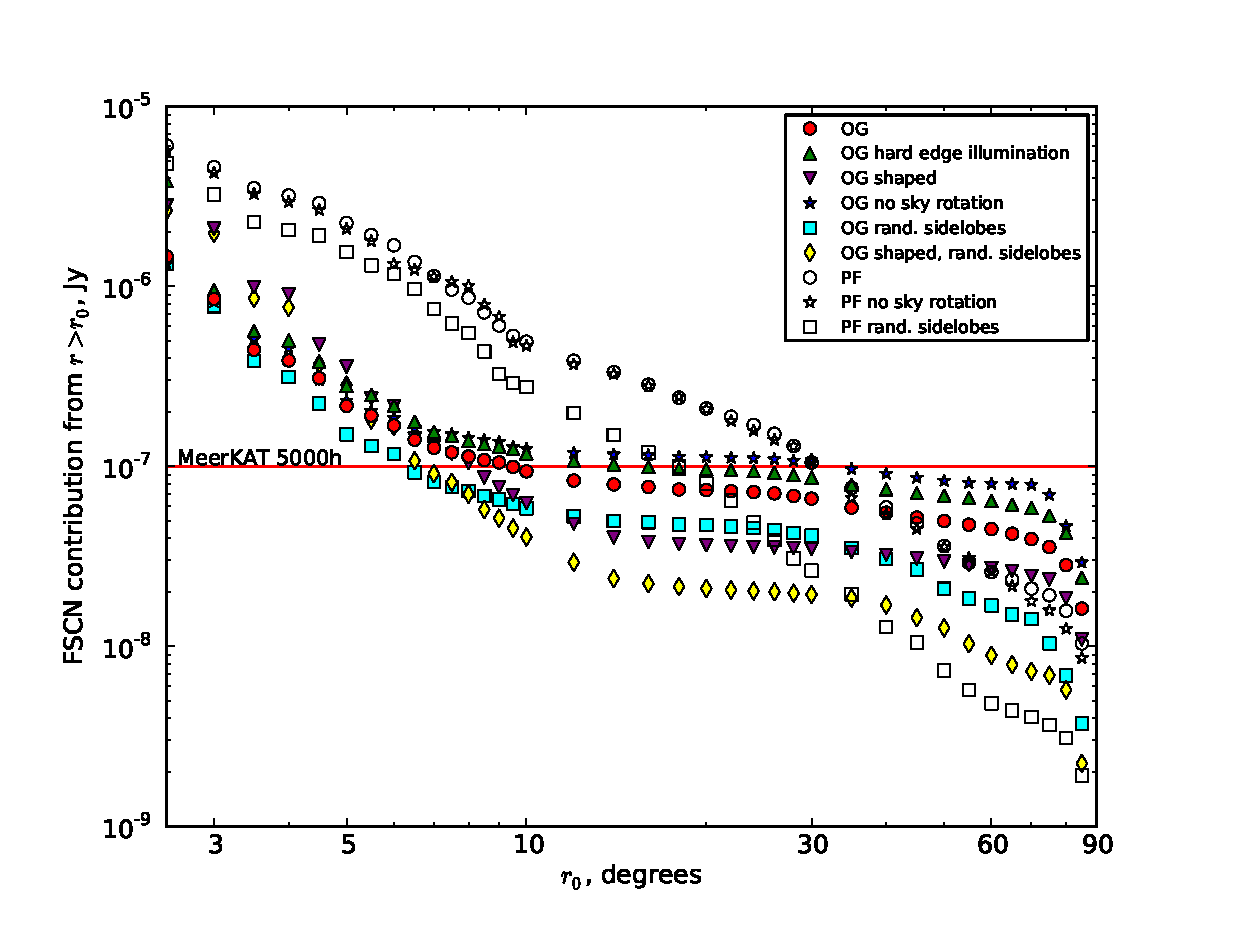
\includegraphics[width=\textwidth]{costcurve-main}
\caption{\label{fig:cc-main}Cost curves: a comparison of FSCN levels as a function of imaging radius, for different MeerKAT dish configurations. The horizontal red line indicates MeerKAT's extreme sensitivity limit for a 5000~h pointing. The plot corresponds to the canonical observational configuration of Sect.~\ref{sec:config}, and a naturally weighted PSF.}
% plot-cc.py horizon-masked/MeerKAT64*natural* -f 10 -t - --x0 1 -a "2.6/1e-7/-/red/-MeerKAT 5000h" --x0 2 --x1 90 -o costcurve-main
% plot-cc.py horizon-masked/MeerKAT64*briggs_r0* -f 10 -t - --x0 1 -a "30/1e-7/-/red/-MeerKAT 5000h" --x0 2 --x1 90 -o costcurve-main-robust
\end{figure*}

The main result for MeerKAT is presented in Fig.~\ref{fig:cc-main}. This contains a number of ``cost curves'' for the various MeerKAT dish options. Each cost curve shows, as a function of $r_0$, the total contribution to the FSCN from sources beyond a radius of $r_0$. It is a \emph{cost} curve because it shows the radius $r_0$ out to which we must image and deconvolve in order to suppress the FSCN to a given level -- and imaging radius directly drives computational cost. 

The most striking feature of this plot is the completely different character of FSCN as a function of $r_0$ for the PF and OG type dishes. The OG curves have an almost flat ``plateau'' between 10$\degr$ and 75$\degr$ (less than a factor of 2 change), while the PF curves maintain nearly constant slope all the way out to 90$\degr$. This is no doubt due to the different dominant features of their PB patterns (Fig.~\ref{fig:pb180}). The PF designs pick up most of their FSCN via the X-shaped sidelobes associated with the feed supports, which are significant at all radii. In contrast, the OG designs pick up a fair chunk of FSCN via the sub-reflector spill-over patch between $75\degr$ and $90\degr$, and then pick up relatively little all the way in to $10\degr$. In other words, as we increase our imaging radius $r_0$, OG designs yield a sharp drop in FSCN until about $10\degr$ -- but once this ``optimal'' radius is reached, increasing $r_0$ further yields very little further improvement, until about $75\degr$. The PF design, on the other hand, shows a much slower but steady decrease in FSCN all the way out to $90\degr$.

A few other interesting points arise from this plot:

\begin{itemize}
  \item This suggests that at MeerKAT's extreme sensitivity limit of $0.1 \mu\mathrm{Jy}$, we must image out to $\sim$10$\degr$ with the default OG dishes, $\sim$20$\degr$ with rotationally randomized PF dishes, and $\sim$30$\degr$ with non-randomized PF dishes (but see the caveat on absolute performance figures below). This is a potentially a massive cost difference!
  \item The OG and PF curves cross over at $\sim$40$\degr$.
  \item Sky rotation makes virtually no difference to the PF design, but provides about a factor of 2 FSCN suppression (beyond $10\degr$) in the OG design.
  \item The shaped OG design starts paying off beyond a radius of $8\degr$, but causes considerably higher FSCN closer in. It is not obvious whether this is a good trade-off or bad, since higher close-in sidelobes can make calibration more difficult.
  \item The hard edge illumination OG design does only slightly worse than the default, to within a factor of 2.
  \item At $10\degr$, sidelobe randomization of OGs does at least a good a job as shaping.
  \item A combination of shaped OGs and sidelobe randomization provides the lowest FSCN levels from $\sim$6$\degr$ out.
  FSCN levels of $0.1 \mu\mathrm{Jy}$ are then achieved by $7\degr$ (provided sidelobe randomization through surface variations can actually be done this close in), which halves the required imaging area, compared to the default OG design. Once again, this has to be weighed against the extra calibration costs associated with higher close-in sidelobes.
\end{itemize}

\subsection{Full sky models and horizon masking}
\label{sec:horizon-masking}




\section{FSCN suppression}

Note that while Fig.~\ref{fig:cc-main} is an excellent indicator of the \emph{relative} performance of the various dish designs, one must be very careful when drawing conclusions on \emph{absolute} performance. The reason for this is that absolute FSCN levels are subject to two other attenuating factors -- see Fig.~2 of \citet{SKA54-expa,SKA54} for a reminder -- which can cause the vertical axis of the cost curves to shifted up and down significantly. Firstly, this is the asymptotic rms PSF sidelobe level, which depends on imaging weights. Secondly, this is the correlator response function $C(r)$, which is determined by time and bandwidth averaging. We shall now consider these two factors in detail.

\subsection{Randomizing PB sidelobes}
\label{sec:randomizing}

A recently developed approach to reducing the FSCN is randomization of PB sidelobes across stations. The LOFAR telescope, in which each station is an aperture array, achieves this via the simple expedient of using a different orientation for the layout of each station. This introduces an essentially random complex gain error for distant sources, thus averaging down their response. Another option for aperture arrays (or indeed PAFs) is to randomize sidelobes by manipulating beamformer weights.

With dishes, PB sidelobes may be randomized in two ways, depending on basic design. A symmetric dish (i.e. the prime focus design) can employ the random rotation trick. This is most likely mechanically prohibitive with an asymmetric design such as the offset Gregorian. Distant sidelobes may also be randomized by introducing small variations in the dish surfaces\footnote{Since the PB is essentially a Fourier transform of the aperture illumination function, far PB sidelobes correspond to small-scale variations in the AIF.}. To a certain extent, the latter happens anyway due to manufacturing tolerances, but may also be done deliberately. Note, however, that the dominant FSCN contribution appears to be associated with the X-shaped sidelobes caused by the feed supports (in the PF case), and the sub-reflector spill-over ``patch'' (in the OG case), neither of which is significantly affected by dish surface variations.

Another intrinsic source of randomization is sky rotation, since over a long synthesis, distant sources will rotate through many sidelobes. This is particularly noticeable with the OG design, where far sidelobes have a checkerboard-like pattern. 

From first principles, we would expect randomization to suppress FSCN as $\sqrt{N}$, where $N$ is the number of stations. Rotational randomization is straightforward to incorporate into the simulations: it is just a matter of introducing a random rotation angle when converting source coordinates in the {\tt emss\_beams} module. This does make for noticeably slower simulations, since E-Jones values then need to be computed individually per station -- unlike the non-randomized case -- but not prohibitively so. We discuss the results in Sects.~\ref{sec:meerkat-costcurve} and \ref{sec:other-arrays}.

\subsection{Effect of imaging weights}
\label{sec:img-weights}

Different imaging weights can be used to optimize the PSF shape for maximum sensitivity (natural weighting), minimum sidelobe level (uniform weighting), or some trade-off between the two \citep[robust or Briggs weighting:][]{briggs-thesis}. Obviously, this directly affects FSCN levels. \citet{SKA49} gives an analytic estimate of asymptotic rms PSF sidelobe levels for natural and uniform weighting. Our simulations allow us to explore this empirically: Fig.~\ref{fig:cc-weights} shows cost curves for the OG and PF designs obtained using natural and uniform weights. Robust weighting produces intermediate curves closer to one or the other extreme, based on the value of the robustness parameter.

\begin{figure}
  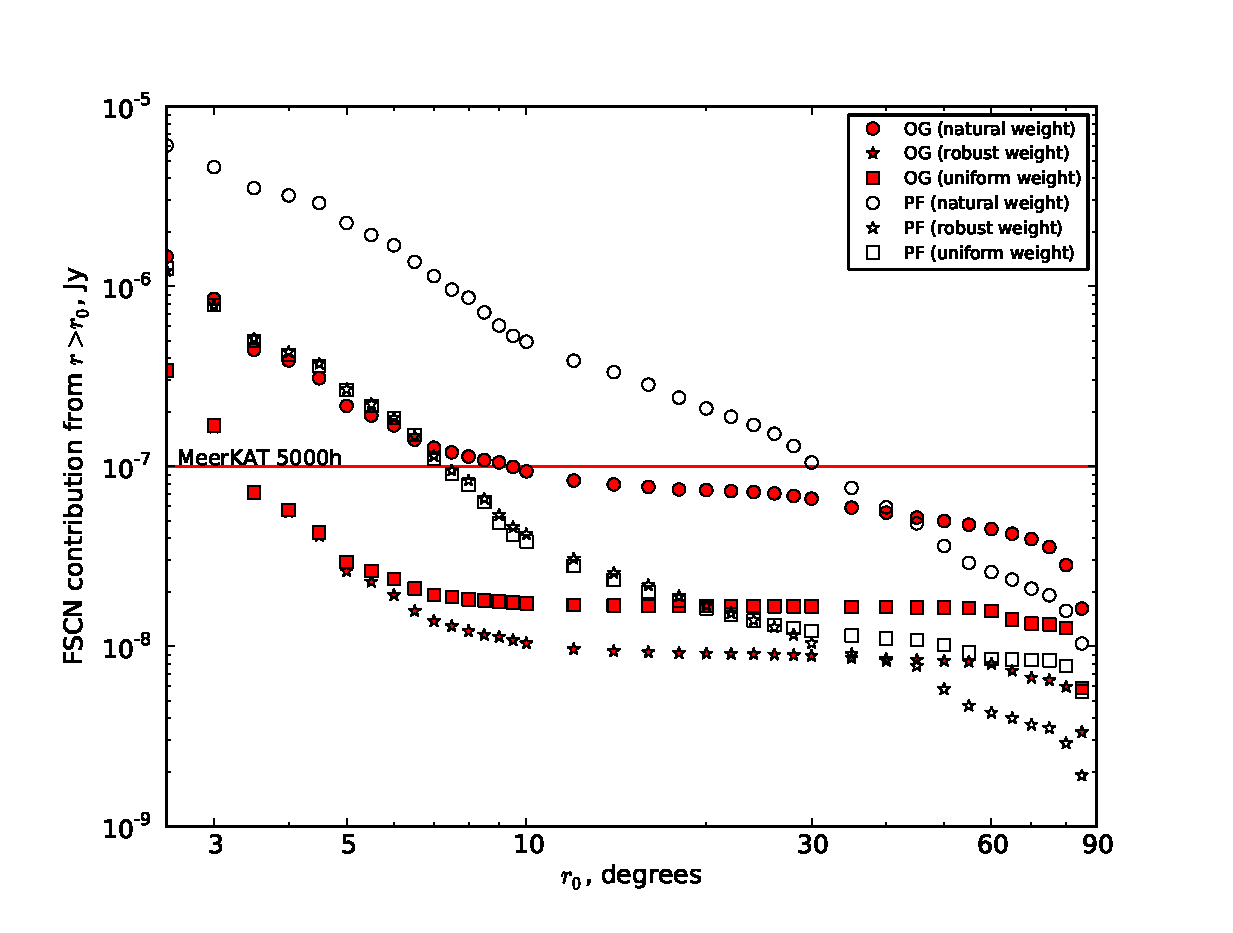
\includegraphics[width=\columnwidth]{cc-mk-nat-vs-uni}
%  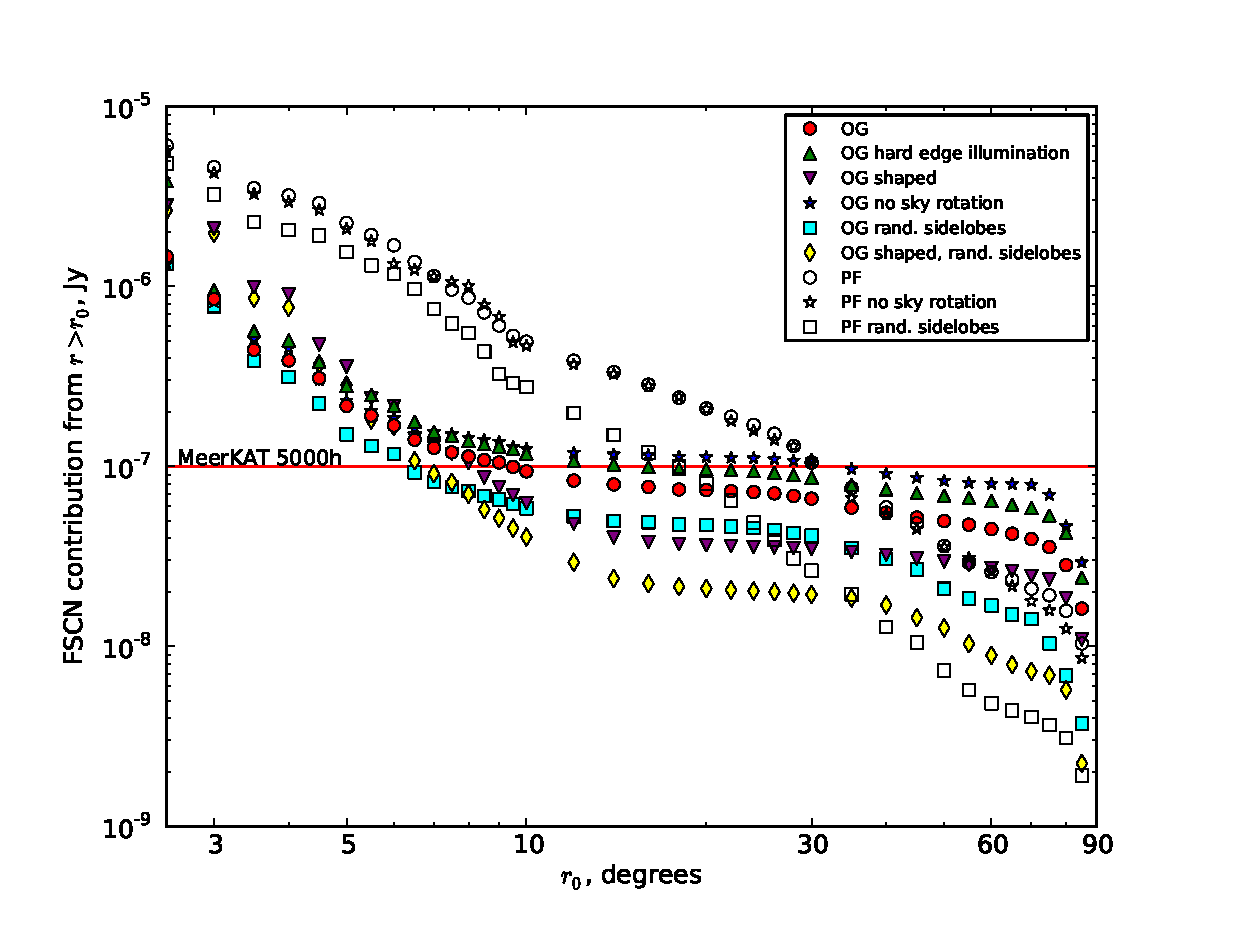
\includegraphics[width=\textwidth]{costcurve-main}
\caption{\label{fig:cc-weights}Cost curves: natural vs. uniform weighting, offset Gregorian vs. prime focus. Observational configuration is the same as in Fig.~\ref{fig:cc-main}, as are the naturally-weighted curves.}
% ../stats-3cbr/plot-cc.py ../stats-3cbr/costs-256pix/MeerKAT64_8h60s_20M8ch_{og,pf}.{natural,uniform}.*  -f 10 -t - --x0 1 -a "2.6/1e-7/-/red/-MeerKAT 5000h" -c a -s w -o cc-mk-nat-vs-uni
\end{figure}

It is to be expected that uniform weighting would suppress the FSCN, though a whole order of magnitude is somewhat surprising (see Sect.~\ref{sec:ifr-size} for a related discussion). Note, however, that this reduction comes at a cost of reduced sensitivity, and that MeerKAT's $0.1\mu$Jy in 5000 hours figure actually assumes natural weighting! Another interesting feature of these curves is that the pay-off of uniform weighting varies as a function of radius, and is slightly higher for the PF design. The effect can be understood by considering  Eq.~(\ref{eq:fscn}) again: this contains an integration over a product of the PSF by the primary beam. The spatial distribution of PSF and PB sidelobes relative to each other can obviously have a large effect. This raises the intriguing possibility that a \emph{joint} optimization of PB shape and PSF shape (and thus array configuration) can produce better FSCN suppression than independent optimization of the two. This ought to be explored further in the context of SKA 
design.

\subsection{Time averaging}
\label{sec:smearing}

Since the correlator produces a complex average over the integration interval, the resulting complex amplitude of each source is attenuated by some factor $C(r)$ \citep[see Eq.~(\ref{eq:fscn}) above, and also Fig.~2 of][]{SKA54-expa,SKA54}. Lonsdale et al. suggest the use of weighted averages within the correlator, as well as baseline-dependent time averaging, as an effective means of FSCN suppression.

The attenuation factor for time averaging follows a sinc function, and strongly depends on baseline length and orientation (or more precisely, the East-West component of the baseline). With each baseline being affected to a different extent, overall FSCN attenuation is difficult to predict analytically, but easy to simulate with our framework, by simply rerunning the same simulation over multiple measurement sets employing different integration times. Since averaging increases with integration time $\Delta t$, intuition suggests that using larger $\Delta t$ should lower the FSCN. In this case intuition misleads -- the curves in Fig.~\ref{fig:cc-time-smearing} show very little difference between the results for $\Delta t=10$, 30 and 60~s!

Such a result appears to directly contradict Lonsdale et al., but in fact the contradiction is easily explained -- those authors considered the case of a snapshot observation, while we are simulating a full (8~hour, in this particular instance) synthesis. \citet{SKA49} showed that (naturally weighted) PSF sidelobes scale approximately as $1/\sqrt{N_s}$, where $N_s$ is the total number of $uv$-samples. However, with larger time bins, we collect fewer $uv$-samples during the same synthesis time, thus increasing PSF sidelobe level as $\sqrt{\Delta t}$. Returning to Eq.~(\ref{eq:fscn}), the drop in $C(r)$ due to longer integrations is then offset by an increase in $P(r)$ due to fewer $uv$-samples. The exact relationship is quite difficult to work out analytically, since one term scales as a sinc function and the other as a square root, but  Fig.~\ref{fig:cc-time-smearing} clearly shows that over the range of feasible MeerKAT integration times, the two terms approximately balance each other out. This also 
suggests that the correlator FoV tailoring technique proposed by Lonsdale et al. will be of limited efficacy for a full synthesis observation.

\subsection{Bandwidth averaging and multi-frequency synthesis}
\label{sec:freq-avg}

Attenuation due to bandwidth averaging has the same underlying cause as that due to time averaging. The basic effect can expected to scale as a sinc function of fractional bandwidth. Figure~\ref{fig:bandwidth-smearing} shows the result of simulations using a single channel of increasing width. The quantity being plotted is the FSCN suppression factor, normalized to unity at 1.25~MHz.

Bandwidth averaging allows for some interesting trade-offs between spectral resolution, sensitivity, and FSCN. Given a frequency band $\Delta\nu_\mathrm{tot}$ split into $N_\mathrm{tot}$ channels, one could choose to average all the channels together prior to imaging, or split the band into sub-bands and average each sub-band, or image each channel separately, or employ multi-frequency synthesis (MFS) with some combination of channel averaging. 

Averaging $n$ channels together suppresses thermal noise by a simple factor of $\sqrt{n}$. FSCN suppression follows the somewhat more complicated sinc-based scaling law of Fig.~\ref{fig:bandwidth-smearing}, and depends on the fractional bandwidth being averaged together, rather than the number of channels per se. Finally, MFS imaging may be employed, which treats each channel (or averaged sub-band) as a separate $uv$-sample, thus reducing PSF sidelobes (see above) and thereby also suppressing FSCN. On the other hand, overly aggressive averaging distorts the resulting images (due to smearing of the Fourier components, and also due to interaction with intrinsic spectral variation of the sources themselves, especially in MFS mode) and destroys spectral information, and thus must be carefully balanced against the science goals of each particular observation.

All this suggests that bandwidth averaging offers a lot of scope for FSCN suppression, but no universal recipe, with different observational regimes benefiting from different trade-offs. The vertical axis of Fig.~\ref{fig:cc-main} can be moved around quite significantly, depending on bandwidth and spectral resolution requirements! In particular, for the two MeerKAT Key Science Projects that intend to reach the extreme sensitivity limit of $0.1\mu$Jy, LADUMA and MIGHTEE {\bf (cite?)}, a more detailed study of this issue should be made.

\section{FSCN for other arrays}
\label{sec:other-arrays}

{\bf NB: this is the old section making comparisons with VLAKAT and WesterKAT. This should be replaced by the MeerKAT16/32/48 comparison, see below}.

Before we can extrapolate any of the present insights to the SKA, we need to develop our understanding of how FSCN scales with array size and layout. Towards this end, we have performed the same simulations on three hypothetical smaller instruments: WesterKAT (14 dishes), VLAKAT (27 dishes) and LOFARKAT (40 dishes). Each of these represents an existing array layout (WSRT, EVLA and LOFAR) shifted to MeerKAT's geographical position, and equipped with MeerKAT dishes. (This was done to keep all other elements of the simulation except array configuration as identical as possible.) We used the same canonical observational configuration described in Sect.~\ref{sec:config}, except for WesterKAT, for which the synthesis time was increased to 12 hours to obtain full $uv$-coverage. 

Table ~\ref{tab:kats} summarizes the various scaling factors of these arrays relative to MeerKAT. (Note that the ratio of the number of $uv$-samples $N_s$ is nominally the same as the ratio of baseline numbers $N_b$, or the square of the ratio of antenna numbers $N_a$, except for WesterKAT, for which the $N_s$ is higher by a factor of 1.5 due to the increased synthesis time.) 

For natural weighting, \citet{SKA49} suggests a scaling law for rms PSF sidelobes of $1/\sqrt{N_s}$, where $N_s$ is the number of $uv$-samples. The number in the last column of Tab.~\ref{tab:kats} gives this number for the other arrays relative to MeerKAT. Can we expect FSCN to scale in the same way? Figs.~\ref{fig:cc-westerkat}--\ref{fig:fscn-rr-suppression} suggest that the answer is a lot more complicated, at least in the smaller array regime. 

% {\bf OMS: I'm finding these figures a little bit mindblowing. There's lots of completely counterintuitive features here, and I think I can even explain some of them (``if you think you understand interferometry, you do not understand interferometry''), but I'd like to have some LOFARKAT sim to fill in the gap first, and completing the MeerKAT-related sections is more urgent. Brad: you need to generate us a LOFARKAT measurement set.}
% 
% \begin{figure}
%   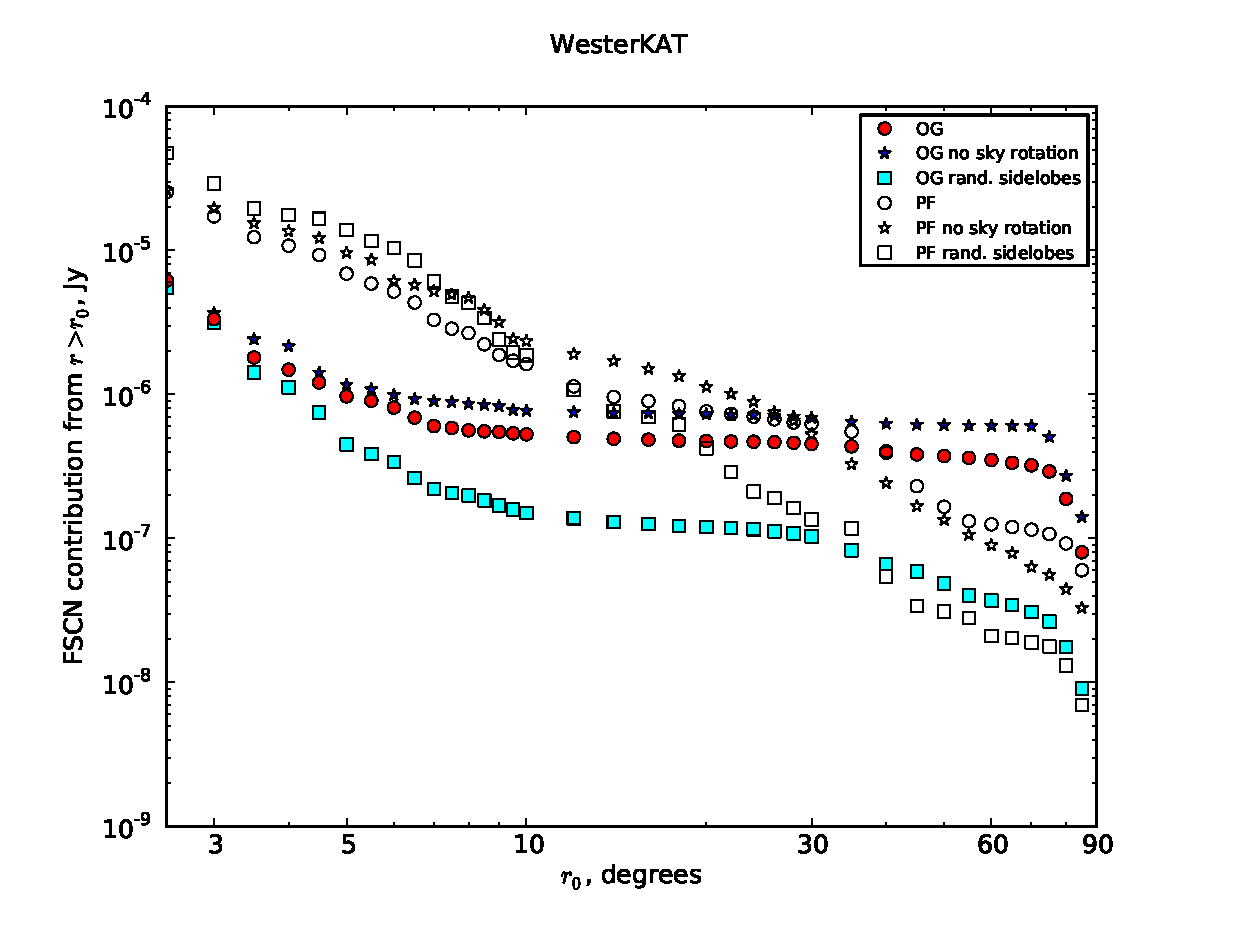
\includegraphics[width=\columnwidth]{cc-westerkat}
%   \caption{\label{fig:cc-westerkat}Cost curves for WesterKAT. The plot corresponds to the canonical observational configuration of Sect.~\ref{sec:config} with a 12~h synthesis, and a naturally weighted PSF.}
% \end{figure}
% \begin{figure}
%   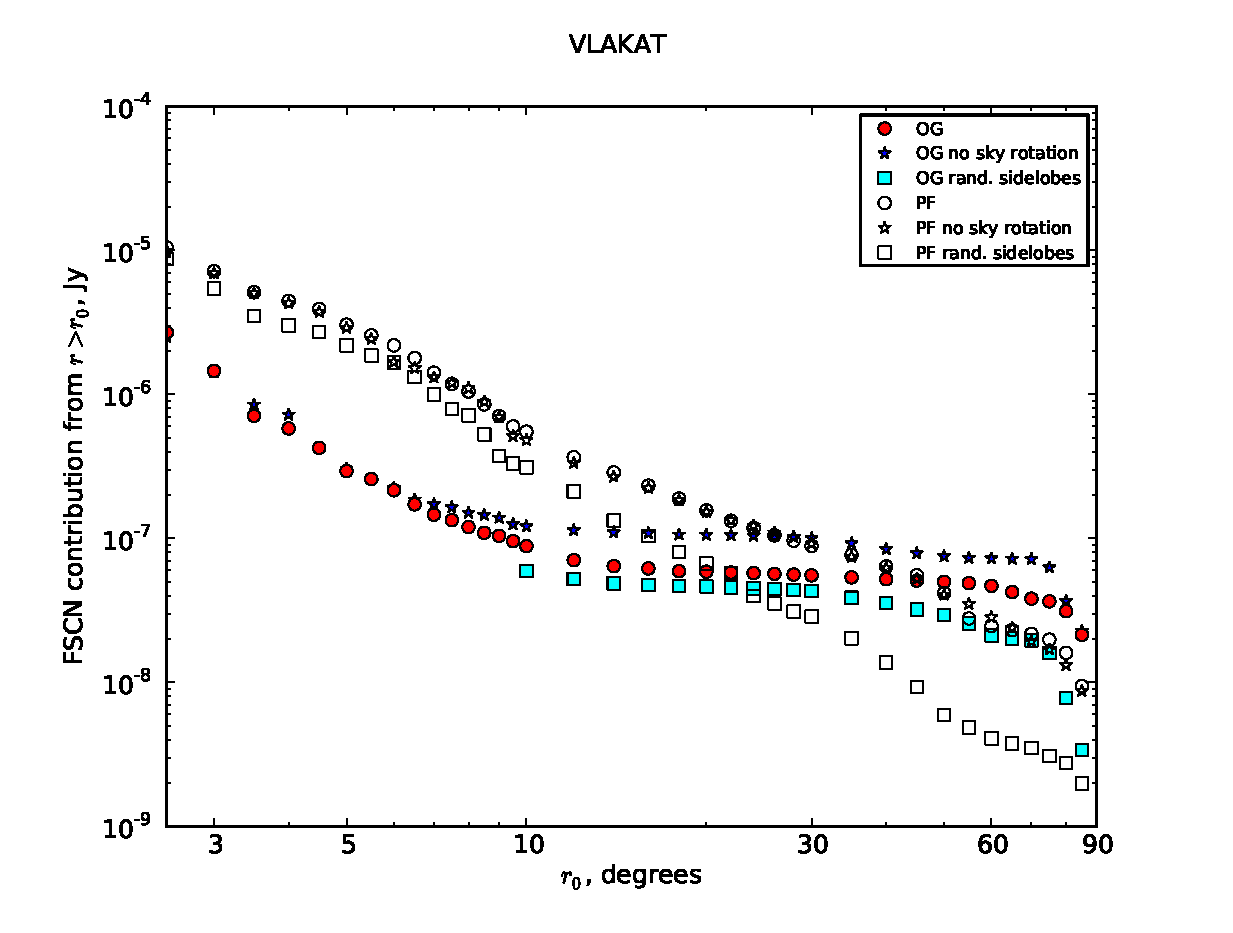
\includegraphics[width=\columnwidth]{cc-vlakat}
%   \caption{\label{fig:cc-vlakat}Cost curves for VLAKAT. The plot corresponds to the canonical observational configuration of Sect.~\ref{sec:config}, and a naturally weighted PSF.}
% \end{figure}
% 
% 
% \begin{table}
% \begin{center}
%   \begin{tabular}[]{lcccccc}
%   \hline
%   \hline
%  & & & & & &\\ [-1ex]
%   & $N_a$ & $\frac{N_{a,\mathrm{MK}}}{N_a}$ & $\sqrt{\frac{N_{a,\mathrm{MK}}}{N_a}}$ & $N_b$ & $\frac{N_{b,\mathrm{MK}}}{N_b}$ & $\sqrt{\frac{N_{s,\mathrm{MK}}}{N_s}}$ \\
%   \hline
%   & & & & & &\\ [-1ex]
% MeerKAT64 & 64 & 1 & 1 & 2016 & 1 & 1 \\
% LOFARKAT & 40 & 1.6 & 1.3 & 780 & 2.6 & 1.6 \\
% VLAKAT & 27 & 2.4 & 1.5 & 351 & 5.7 & 2.4 \\
% WesterKAT & 14 & 4.6 & 2.1 & 91 & 22.2 & 3.8 \\
%   \hline
%   \end{tabular}
% \end{center}
% \caption{\label{tab:kats}Various scaling fractions for our simulated arrays. $N_a$ is the number of antennas, $N_b$ is the number of baselines, and $N_s$ is the number of $uv$-samples. The fractions are relative to the MeerKAT64 numbers.}
% \end{table}
% 
% 
% \begin{figure*}
%   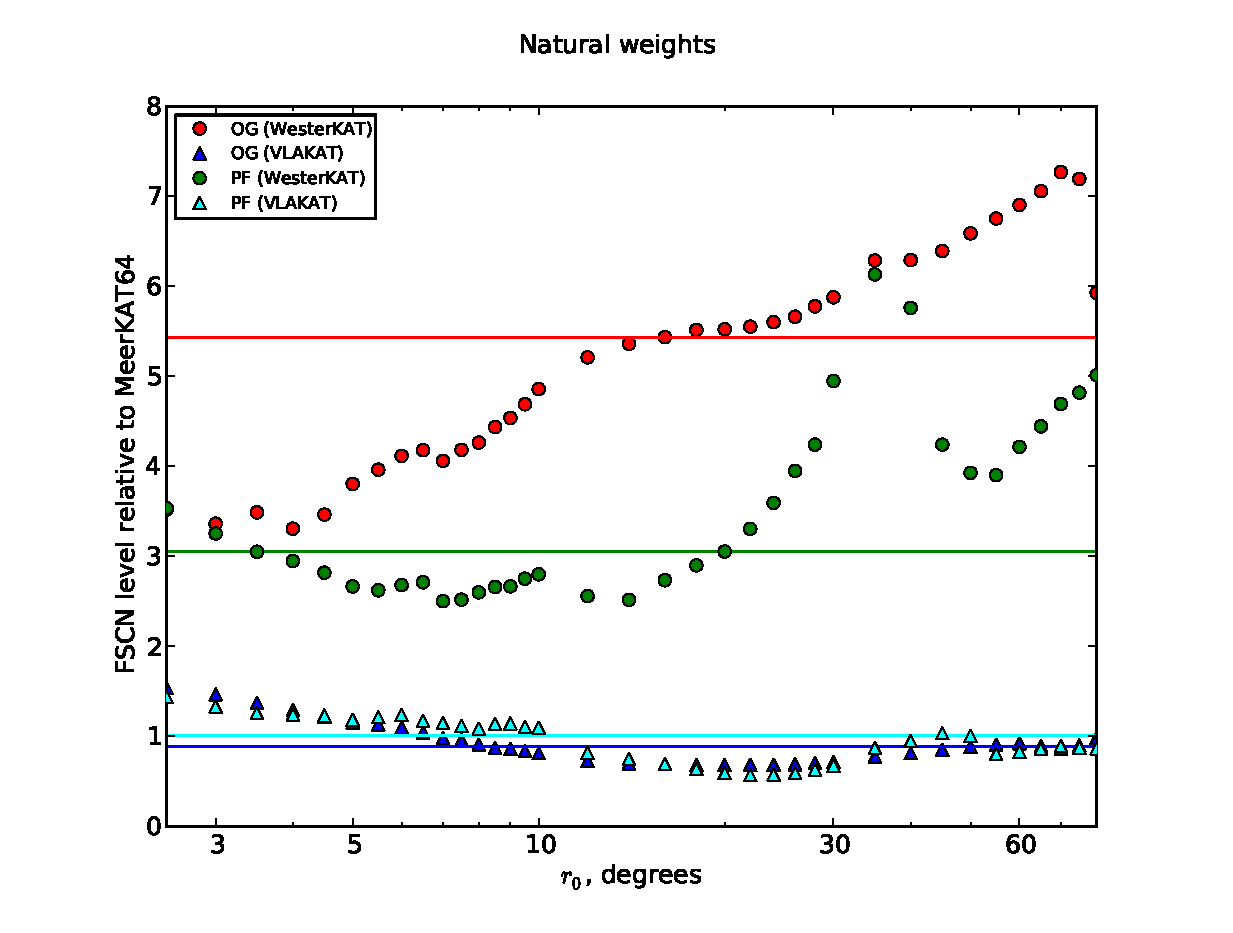
\includegraphics[width=\columnwidth]{cc-multiobs-frac-natural}
%   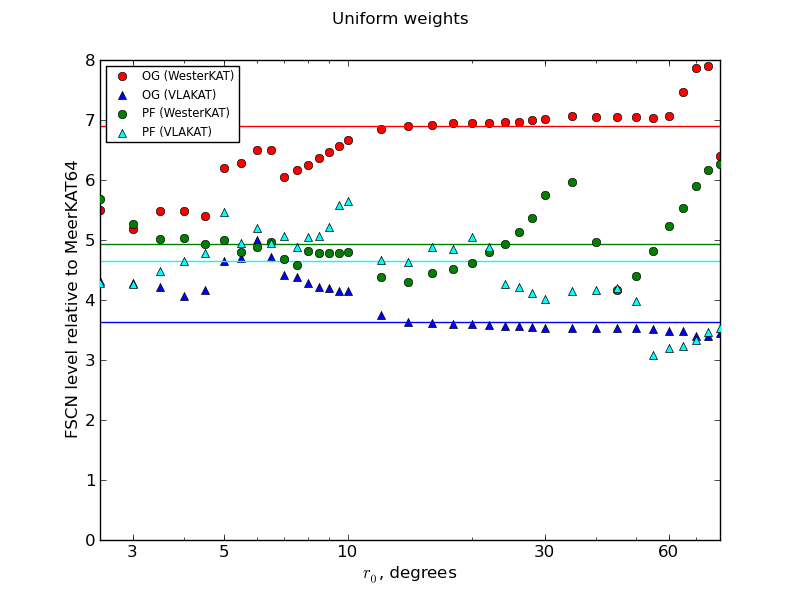
\includegraphics[width=\columnwidth]{cc-multiobs-frac-uniform}
% %  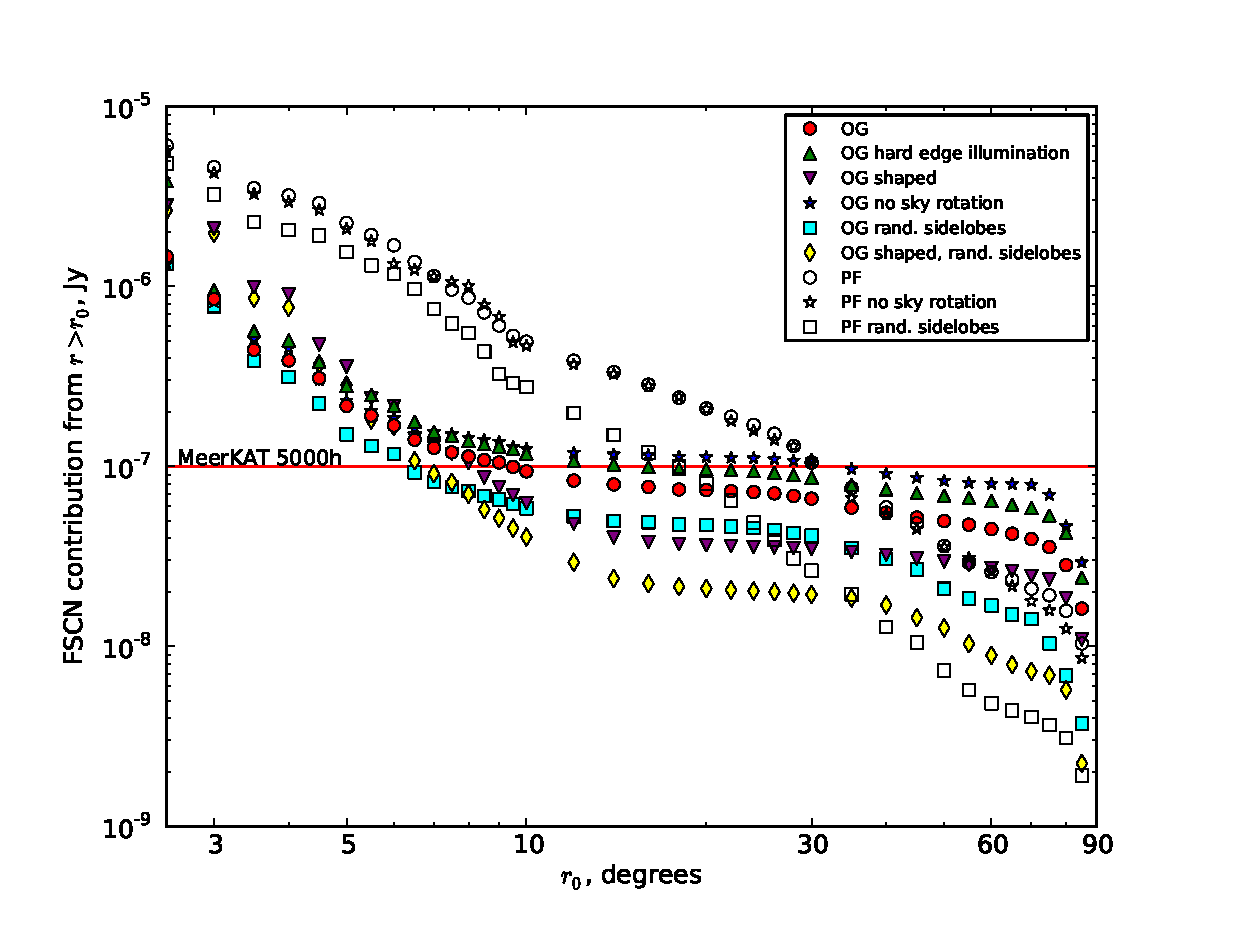
\includegraphics[width=\textwidth]{costcurve-main}
% \caption{\label{fig:fscn-relative}FSCN levels of smaller arrays, normalized to MeerKAT64 levels. Horizontal lines correspond to median values.}
% %  ./plot-cc.py WesterKAT_12h60s_20M8ch_og_natural_no_wproj.txt MeerKAT64_8h60s_20M8ch_og_natural_no_wproj.txt VLAKAT_8h60s_20M8ch_og_natural_no_wproj.txt MeerKAT64_8h60s_20M8ch_og_natural_no_wproj.txt WesterKAT_12h60s_20M8ch_pf_natural_no_wproj.txt MeerKAT64_8h60s_20M8ch_pf_natural_no_wproj.txt costs-256pix/VLAKAT_8h60s_20M8ch_pf.natural.cost.txt MeerKAT64_8h60s_20M8ch_pf_natural_no_wproj.txt -f 10 -s a -c n -o cc-multiobs-frac-natural -n --r1 80 -y "FSCN level relative to MeerKAT64" -p "upper left" --y0 0 -t "Natural weights" -M
% %  ./plot-cc.py costs-256pix/WesterKAT_12h60s_20M8ch_og.uniform.cost.txt costs-256pix/MeerKAT64_8h60s_20M8ch_og.uniform.cost.txt costs-256pix/VLAKAT_8h60s_20M8ch_og.uniform.cost.txt costs-256pix/MeerKAT64_8h60s_20M8ch_og.uniform.cost.txt costs-256pix/WesterKAT_12h60s_20M8ch_pf.uniform.cost.txt costs-256pix/MeerKAT64_8h60s_20M8ch_pf.uniform.cost.txt costs-256pix/VLAKAT_8h60s_20M8ch_pf.uniform.cost.txt costs-256pix/MeerKAT64_8h60s_20M8ch_pf.uniform.cost.txt -f 10 -s a -c n -o cc-multiobs-frac-uniform -n --r1 80 -y "FSCN level relative to MeerKAT64" -p "upper left" --y0 0 -t "Uniform weights" -M
% \end{figure*}
% 
% 
% \begin{figure*}
%   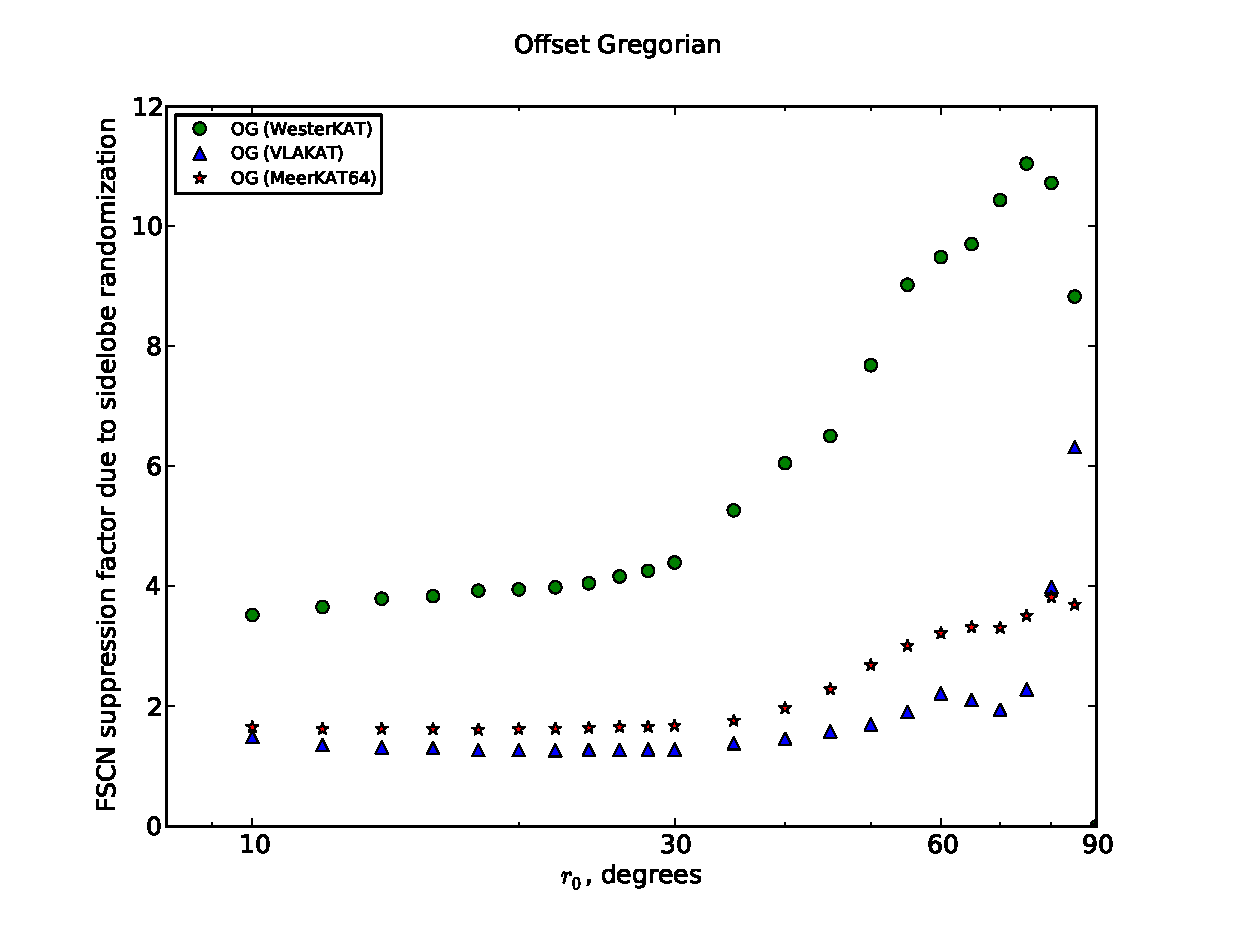
\includegraphics[width=\columnwidth]{rr-suppression-og}
%   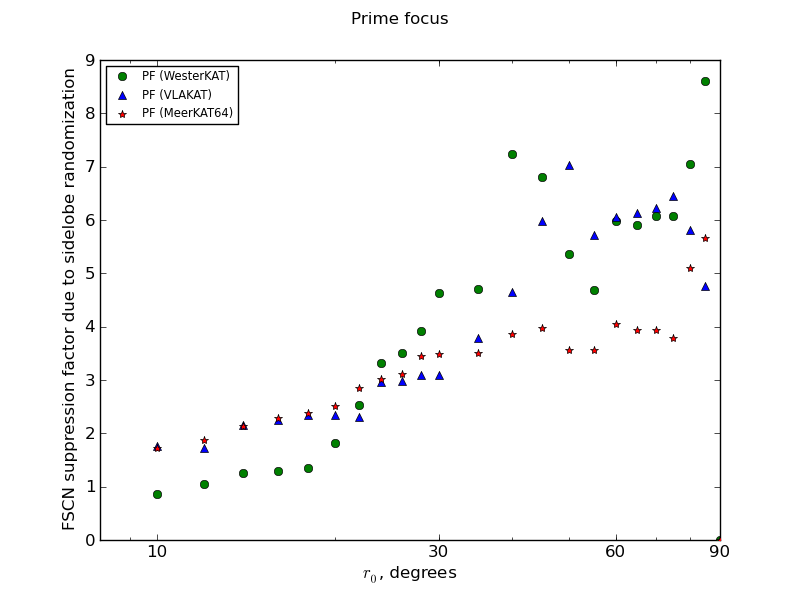
\includegraphics[width=\columnwidth]{rr-suppression-pf}
% %  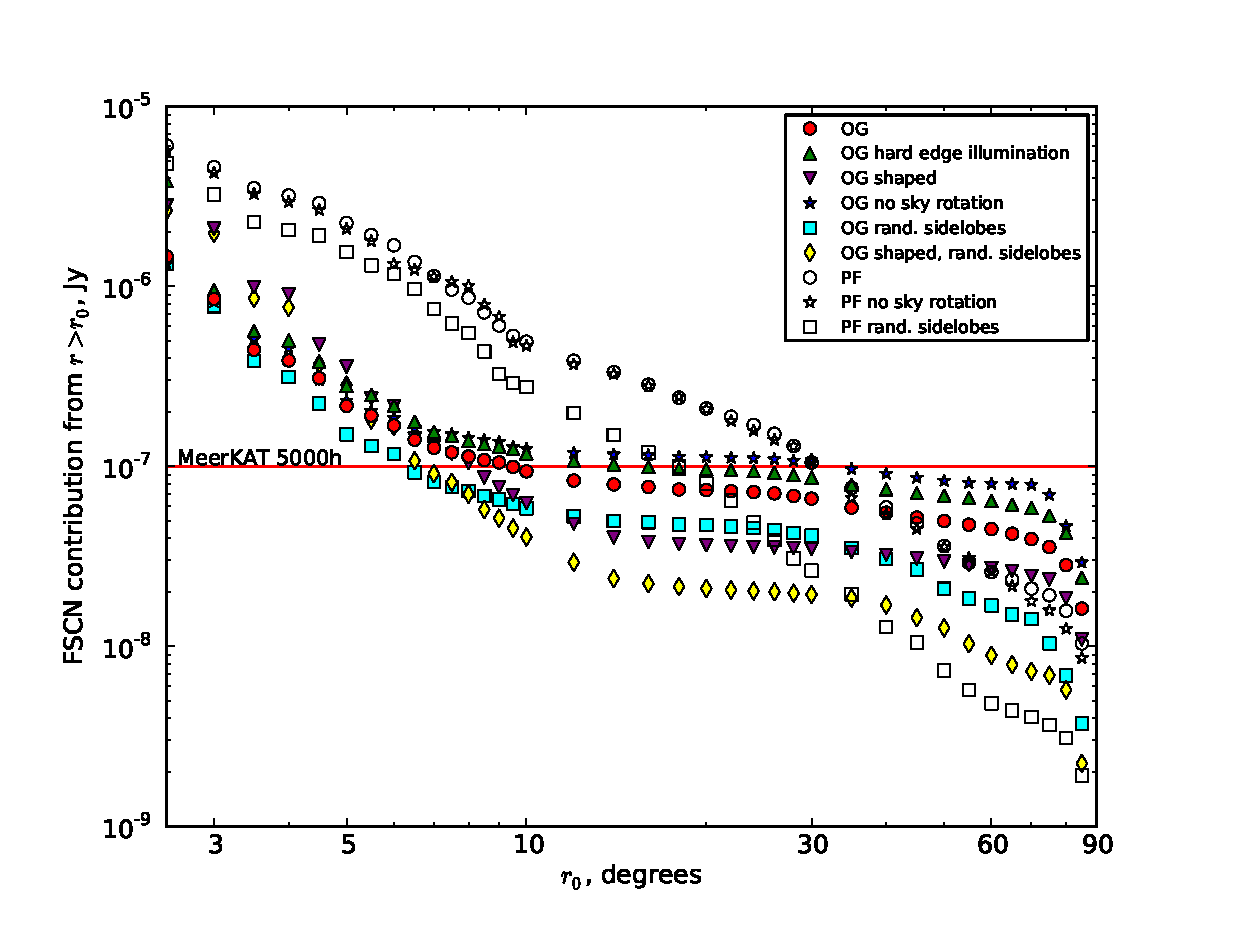
\includegraphics[width=\textwidth]{costcurve-main}
% \caption{\label{fig:fscn-rr-suppression}FSCN suppression factor due to sidelobe randomization, for OG and PF designs.}
% %./plot-cc.py costs-2048pix-no_wproj/WesterKAT_12h60s_20M8ch_pf.natural.txt costs-2048pix-no_wproj/WesterKAT_12h60s_20M8ch_pf_rr.natural.txt costs-2048pix-no_wproj/VLAKAT_8h60s_20M8ch_pf.natural.txt costs-2048pix-no_wproj/VLAKAT_8h60s_20M8ch_pf_rr.natural.txt costs-2048pix-no_wproj/MeerKAT64_8h60s_20M8ch_pf.natural.txt costs-2048pix-no_wproj/MeerKAT64_8h60s_20M8ch_pf_rr.natural.txt -n --r0 10 --x0 8 -y "FSCN suppression factor due to sidelobe randomization" --title "Prime focus" -p "upper left" -o "rr-suppression-pf"
% %./plot-cc.py costs-2048pix-no_wproj/WesterKAT_12h60s_20M8ch_og.natural.txt costs-2048pix-no_wproj/WesterKAT_12h60s_20M8ch_og_rr.natural.txt costs-2048pix-no_wproj/VLAKAT_8h60s_20M8ch_og.natural.txt costs-2048pix-no_wproj/VLAKAT_8h60s_20M8ch_og_rr.natural.txt costs-2048pix-no_wproj/MeerKAT64_8h60s_20M8ch_og.natural.txt costs-2048pix-no_wproj/MeerKAT64_8h60s_20M8ch_og_rr.natural.txt -n --r0 10 --x0 8 -y "FSCN suppression factor due to sidelobe randomization" --title "Offset Gregorian" -p "upper left" -o "rr-suppression-og"
% \end{figure*}

\section{FSCN scaling with array size}
\label{sec:meerkatjes}

\begin{figure*}
  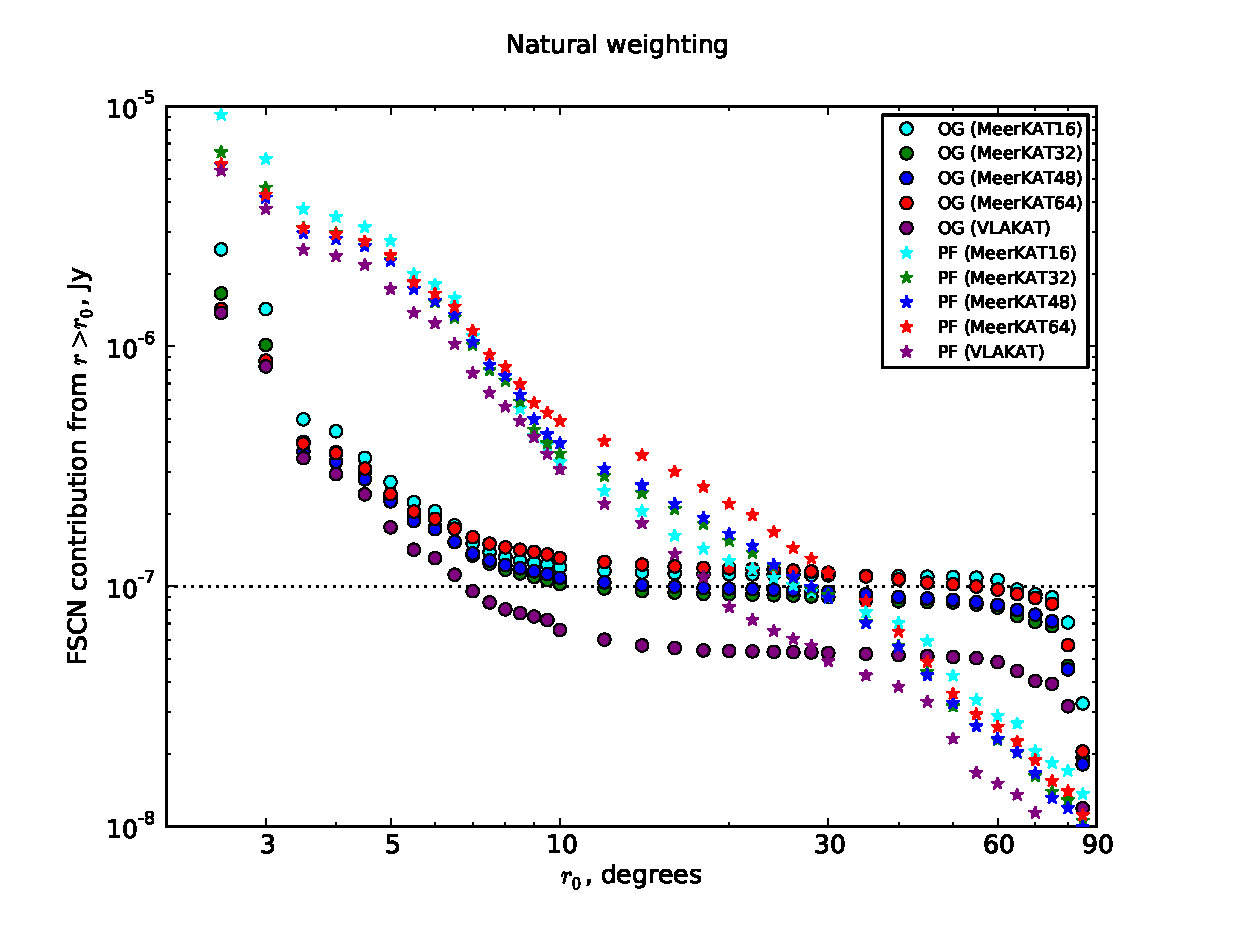
\includegraphics[width=.33\textwidth]{cc-meerkatjes-natural}\hfill%
  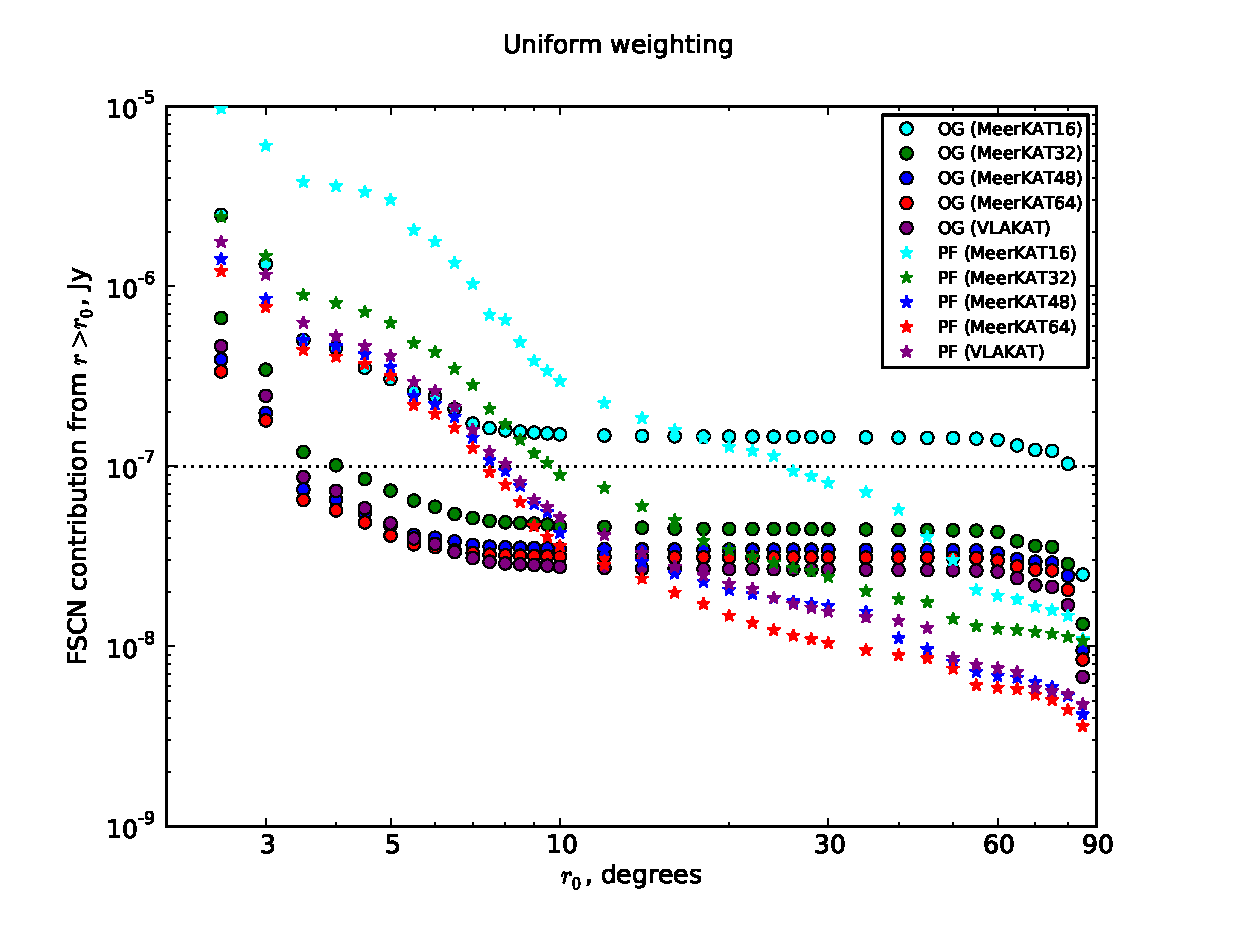
\includegraphics[width=.33\textwidth]{cc-meerkatjes-uniform}\hfill%
  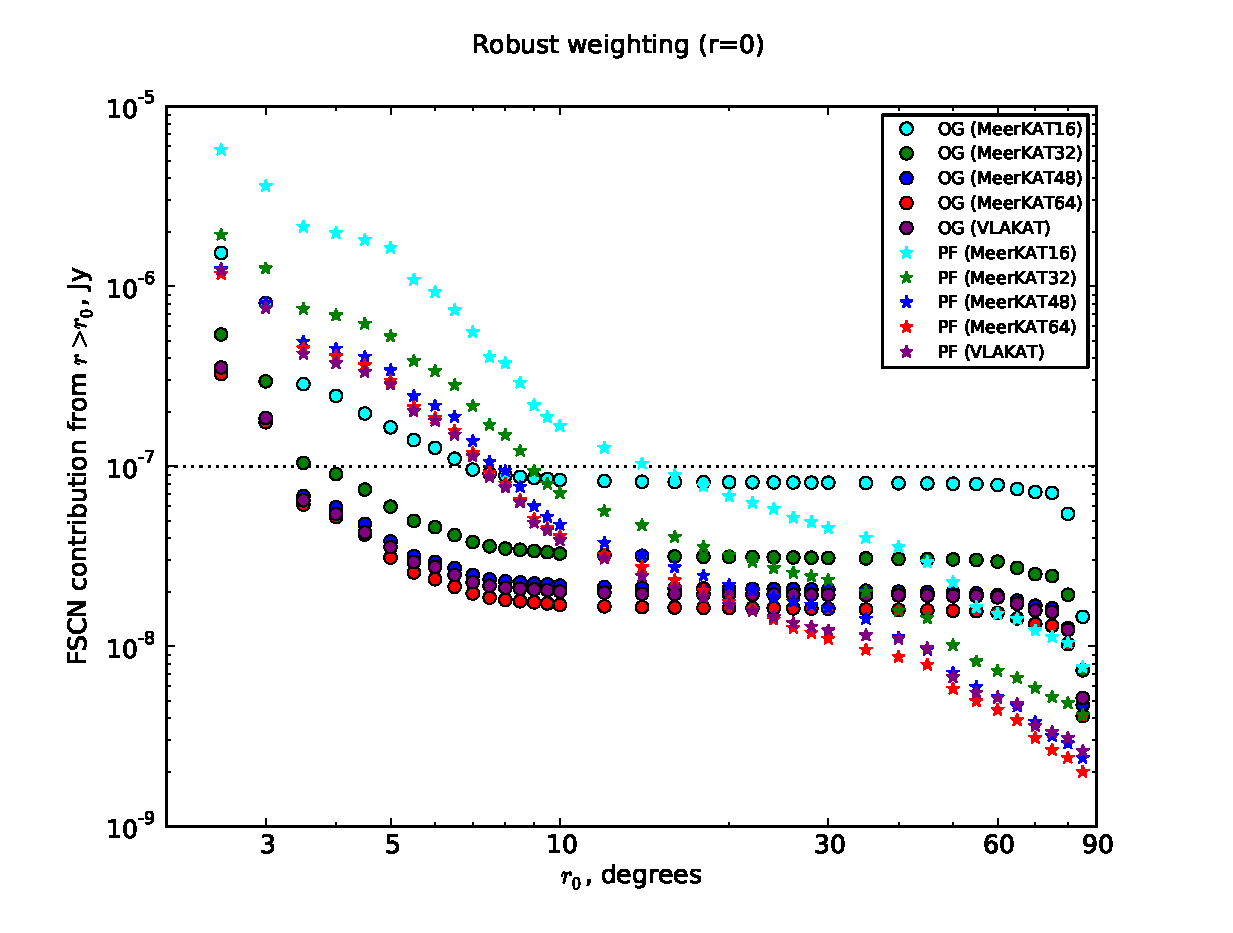
\includegraphics[width=.33\textwidth]{cc-meerkatjes-robust}
\caption{\label{fig:fscn-meerkatjes}FSCN levels for smaller MeerKATs, for OG and PF designs. Note how the naturally-weighted FSCN levels do not really scale down with array size.}
%./plot-cc.py costs/MK{16,32,48,64}/*{pf,og}.natural* costs/VLAKAT/*{pf,og}.natural* -f 10 -t "Natural weighting" --x0 2 --x1 90 -o cc-meerkatjes-natural -s D -a 0/1e-7/:/black/ --y0 1e-8 --y1 1e-5
%./plot-cc.py costs/MK{16,32,48,64}/*{pf,og}.briggs_r_2* costs/VLAKAT/*{pf,og}.briggs_r_2* -f 10 -t "Uniform weighting" --x0 2 --x1 90 -o cc-meerkatjes-uniform -s D -a 0/1e-7/:/black/ --y0 1e-9 --y1 1e-5
%./plot-cc.py costs/MK{16,32,48,64}/*{pf,og}.briggs_r0* costs/VLAKAT/*{pf,og}.briggs_r0* -f 10 -t "Robust weighting (r=0)" --x0 2 --x1 90 -o cc-meerkatjes-robust -s D -a 0/1e-7/:/black/ --y0 1e-9 --y1 1e-5

\end{figure*}

\begin{figure*}
  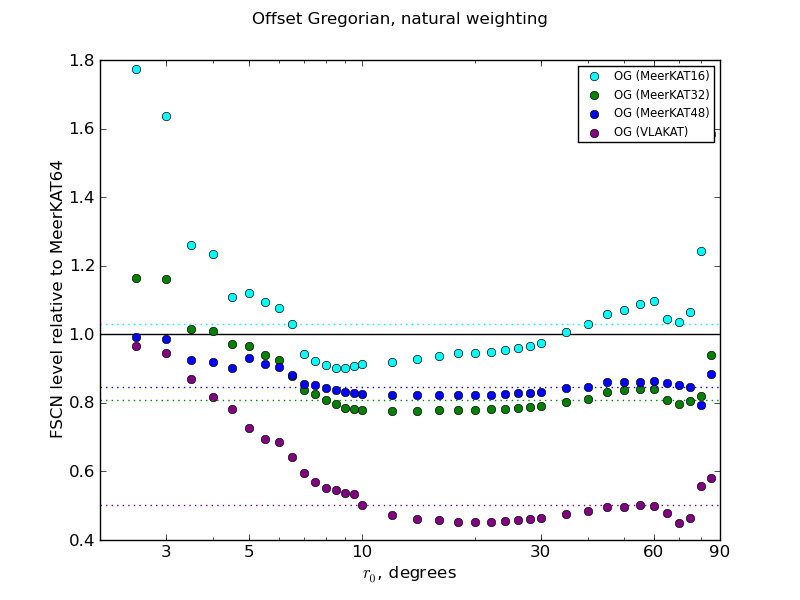
\includegraphics[width=.33\textwidth]{cc-meerkatjes-ratio-og-nat}\hfill%
  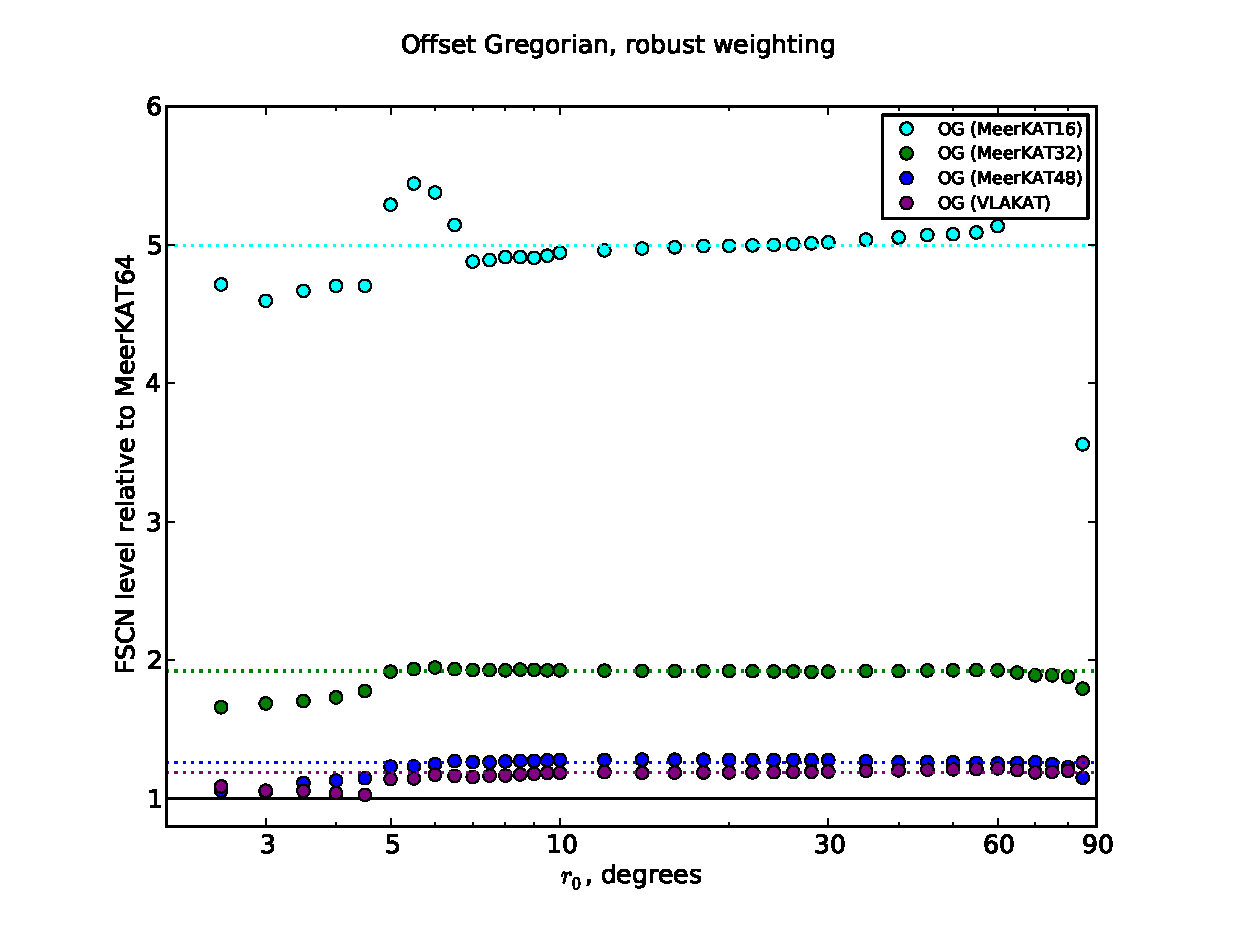
\includegraphics[width=.33\textwidth]{cc-meerkatjes-ratio-og}\hfill%
  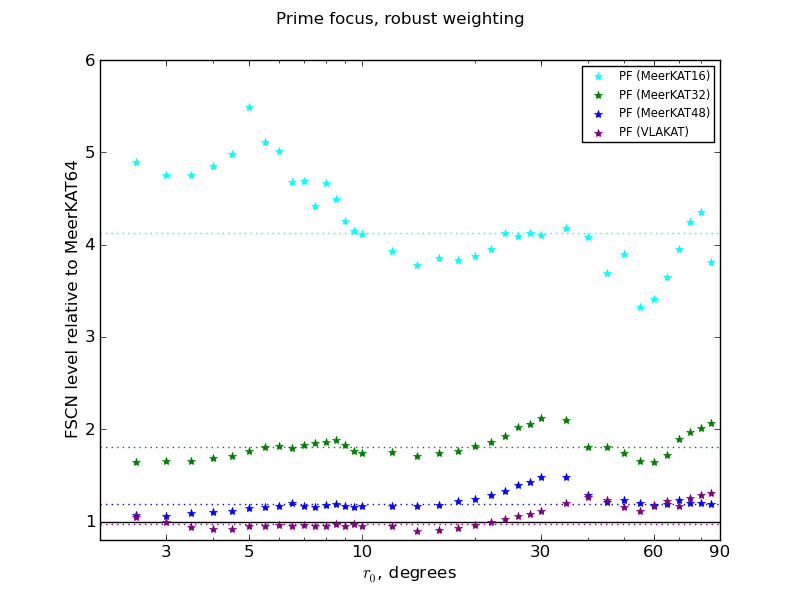
\includegraphics[width=.33\textwidth]{cc-meerkatjes-ratio-pf}
\caption{\label{fig:fscn-meerkatjes-relative}Relative FSCN levels for smaller MeerKATs, for OG and PF designs, normalized to the MeerKAT64 level. Note how surprisingly well VLAKAT does!}
%1; weight=natural; dish=og; ./plot-cc.py costs/MK16/MeerKAT16_8h60s_20M8ch_${dish}.${weight}*txt costs/MK64/MeerKAT64_8h60s_20M8ch_${dish}.${weight}*txt costs/MK32/MeerKAT32_8h60s_20M8ch_${dish}.${weight}*txt costs/MK64/MeerKAT64_8h60s_20M8ch_${dish}.${weight}*txt costs/MK48/MeerKAT48_8h60s_20M8ch_${dish}.${weight}*txt costs/MK64/MeerKAT64_8h60s_20M8ch_${dish}.${weight}*txt costs/VLAKAT/VLAKAT_8h60s_20M8ch_${dish}.${weight}*txt  costs/MK64/MeerKAT64_8h60s_20M8ch_${dish}.${weight}*txt -n -f 10 -t "Offset Gregorian, natural weighting" --x0 2 --x1 90 -o cc-meerkatjes-ratio-${dish}-nat -y "FSCN level relative to MeerKAT64" -s D -a 0/1/-/black/ -c a -M
%2; weight=briggs_r0; dish=og; ./plot-cc.py costs/MK16/MeerKAT16_8h60s_20M8ch_${dish}.${weight}*txt costs/MK64/MeerKAT64_8h60s_20M8ch_${dish}.${weight}*txt costs/MK32/MeerKAT32_8h60s_20M8ch_${dish}.${weight}*txt costs/MK64/MeerKAT64_8h60s_20M8ch_${dish}.${weight}*txt costs/MK48/MeerKAT48_8h60s_20M8ch_${dish}.${weight}*txt costs/MK64/MeerKAT64_8h60s_20M8ch_${dish}.${weight}*txt costs/VLAKAT/VLAKAT_8h60s_20M8ch_${dish}.${weight}*txt  costs/MK64/MeerKAT64_8h60s_20M8ch_${dish}.${weight}*txt -n -f 10 -t "Offset Gregorian, robust weighting" --x0 2 --x1 90 -o cc-meerkatjes-ratio-${dish} -y "FSCN level relative to MeerKAT64" -s D -a 0/1/-/black/ -c a -M --y0 0.8 --y1 6 
%3; weight=briggs_r0; dish=pf; ./plot-cc.py costs/MK16/MeerKAT16_8h60s_20M8ch_${dish}.${weight}*txt costs/MK64/MeerKAT64_8h60s_20M8ch_${dish}.${weight}*txt costs/MK32/MeerKAT32_8h60s_20M8ch_${dish}.${weight}*txt costs/MK64/MeerKAT64_8h60s_20M8ch_${dish}.${weight}*txt costs/MK48/MeerKAT48_8h60s_20M8ch_${dish}.${weight}*txt costs/MK64/MeerKAT64_8h60s_20M8ch_${dish}.${weight}*txt costs/VLAKAT/VLAKAT_8h60s_20M8ch_${dish}.${weight}*txt  costs/MK64/MeerKAT64_8h60s_20M8ch_${dish}.${weight}*txt -n -f 10 -t "Prime focus, robust weighting" --x0 2 --x1 90 -o cc-meerkatjes-ratio-${dish} -y "FSCN level relative to MeerKAT64" -s D -a 0/1/-/black/ -c a -M --y0 0.8 --y1 6 
\end{figure*}

\begin{figure*}
  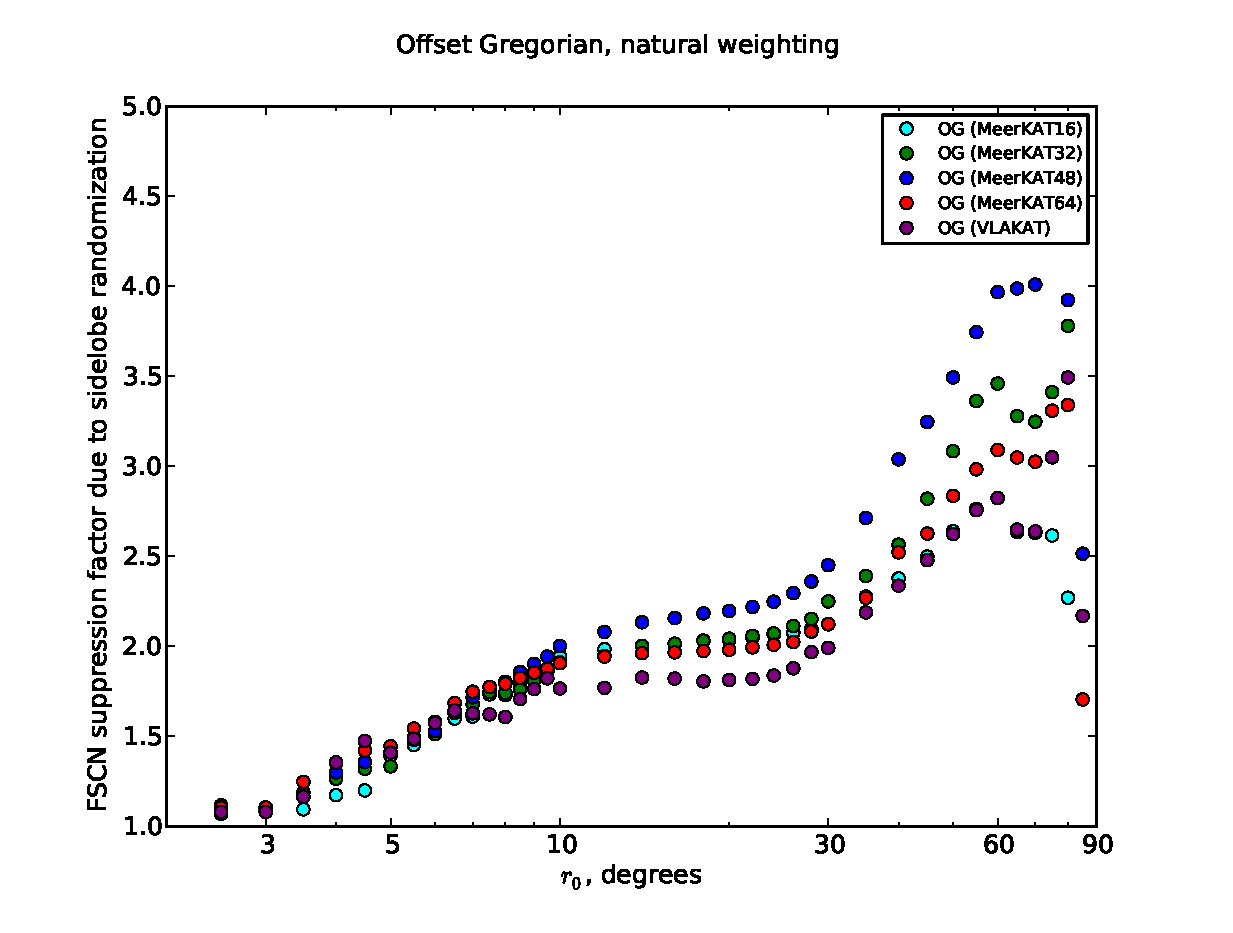
\includegraphics[width=.33\textwidth]{cc-meerkatjes-rrsupp-og-nat}\hfill%
  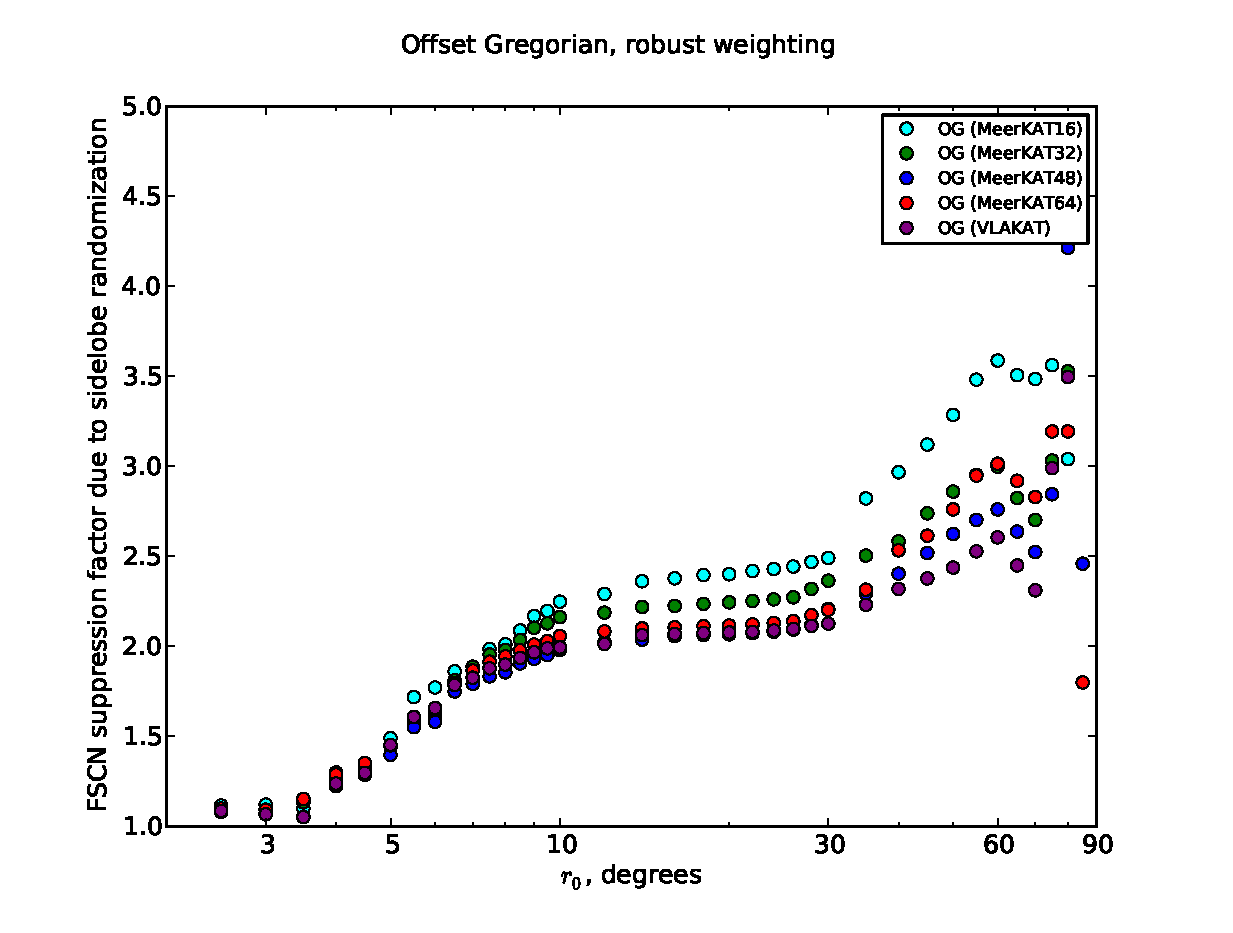
\includegraphics[width=.33\textwidth]{cc-meerkatjes-rrsupp-og}\hfill%
  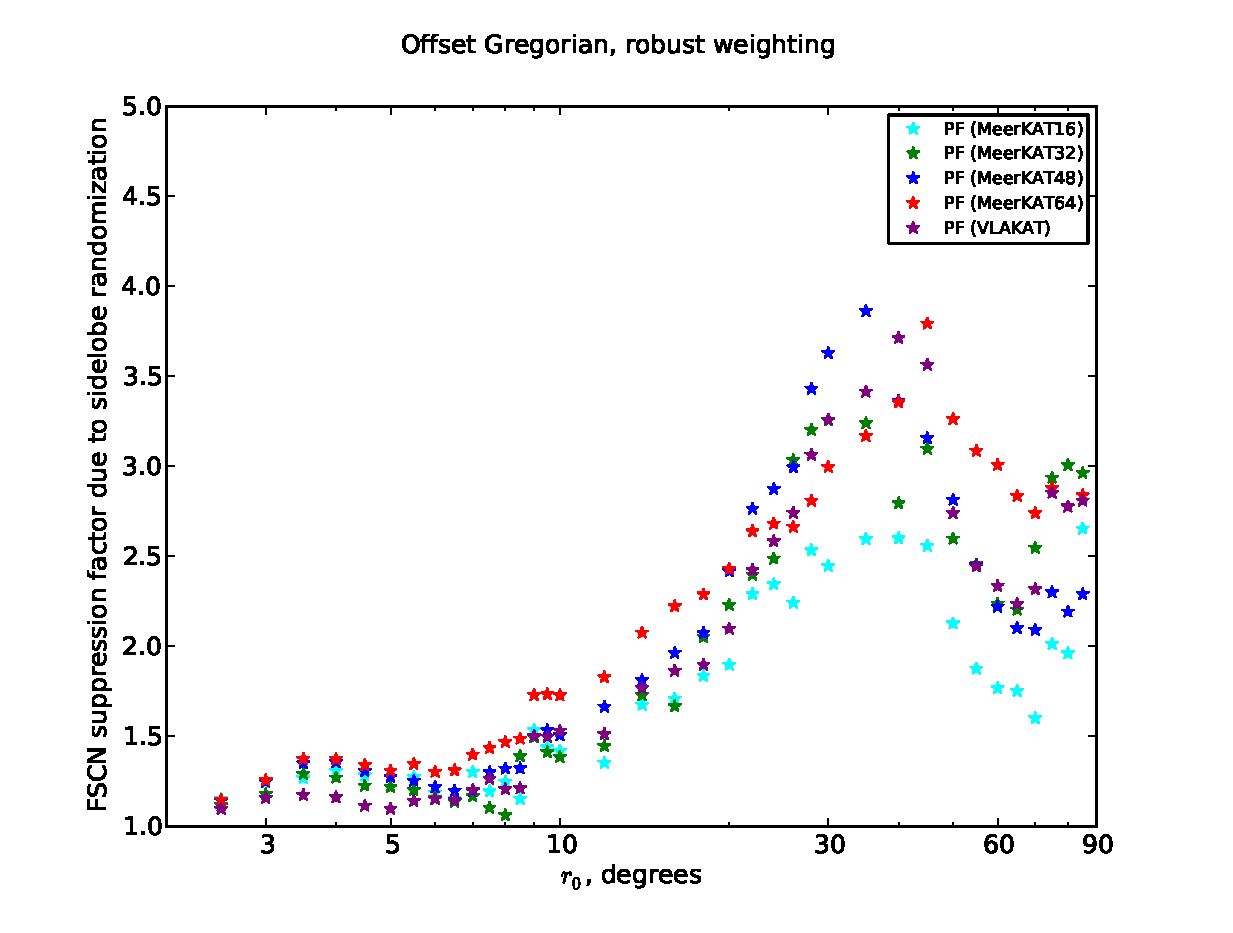
\includegraphics[width=.33\textwidth]{cc-meerkatjes-rrsupp-pf}
\caption{\label{fig:fscn-meerkatjes-rr-suppression}FSCN suppression factor due to sidelobe randomization, for OG and PF designs.}
%3; weight=natural; dish=og; ./plot-cc.py costs/MK16/MeerKAT16_8h60s_20M8ch_${dish}.${weight}*txt costs/MK16/MeerKAT16_8h60s_20M8ch_${dish}_rr.${weight}*txt costs/MK32/MeerKAT32_8h60s_20M8ch_${dish}.${weight}*txt costs/MK32/MeerKAT32_8h60s_20M8ch_${dish}_rr.${weight}*txt costs/MK48/MeerKAT48_8h60s_20M8ch_${dish}.${weight}*txt costs/MK48/MeerKAT48_8h60s_20M8ch_${dish}_rr.${weight}*txt costs/MK64/MeerKAT64_8h60s_20M8ch_${dish}.${weight}*txt costs/MK64/MeerKAT64_8h60s_20M8ch_${dish}_rr.${weight}*txt costs/VLAKAT/VLAKAT_8h60s_20M8ch_${dish}.${weight}*txt costs/VLAKAT/VLAKAT_8h60s_20M8ch_${dish}_rr.${weight}*txt -n -f 10 -t "Offset Gregorian, natural weighting" --x0 2 --x1 90 -o cc-meerkatjes-rrsupp-${dish}-nat -y "FSCN suppression factor due to sidelobe randomization" -s D -a 0/1/-/black/ -c a --y0 1 --y1 5
%3; weight=briggs_r0; dish=og; ./plot-cc.py costs/MK16/MeerKAT16_8h60s_20M8ch_${dish}.${weight}*txt costs/MK16/MeerKAT16_8h60s_20M8ch_${dish}_rr.${weight}*txt costs/MK32/MeerKAT32_8h60s_20M8ch_${dish}.${weight}*txt costs/MK32/MeerKAT32_8h60s_20M8ch_${dish}_rr.${weight}*txt costs/MK48/MeerKAT48_8h60s_20M8ch_${dish}.${weight}*txt costs/MK48/MeerKAT48_8h60s_20M8ch_${dish}_rr.${weight}*txt costs/MK64/MeerKAT64_8h60s_20M8ch_${dish}.${weight}*txt costs/MK64/MeerKAT64_8h60s_20M8ch_${dish}_rr.${weight}*txt costs/VLAKAT/VLAKAT_8h60s_20M8ch_${dish}.${weight}*txt costs/VLAKAT/VLAKAT_8h60s_20M8ch_${dish}_rr.${weight}*txt  -n -f 10 -t "Offset Gregorian, robust weighting" --x0 2 --x1 90 -o cc-meerkatjes-rrsupp-${dish} -y "FSCN suppression factor due to sidelobe randomization" -s D -a 0/1/-/black/ -c a --y0 1 --y1 5
%3; weight=briggs_r0; dish=pf; ./plot-cc.py costs/MK16/MeerKAT16_8h60s_20M8ch_${dish}.${weight}*txt costs/MK16/MeerKAT16_8h60s_20M8ch_${dish}_rr.${weight}*txt costs/MK32/MeerKAT32_8h60s_20M8ch_${dish}.${weight}*txt costs/MK32/MeerKAT32_8h60s_20M8ch_${dish}_rr.${weight}*txt costs/MK48/MeerKAT48_8h60s_20M8ch_${dish}.${weight}*txt costs/MK48/MeerKAT48_8h60s_20M8ch_${dish}_rr.${weight}*txt costs/MK64/MeerKAT64_8h60s_20M8ch_${dish}.${weight}*txt costs/MK64/MeerKAT64_8h60s_20M8ch_${dish}_rr.${weight}*txt costs/VLAKAT/VLAKAT_8h60s_20M8ch_${dish}.${weight}*txt costs/VLAKAT/VLAKAT_8h60s_20M8ch_${dish}_rr.${weight}*txt  -n -f 10 -t "Offset Gregorian, robust weighting" --x0 2 --x1 90 -o cc-meerkatjes-rrsupp-${dish} -y "FSCN suppression factor due to sidelobe randomization" -s D -a 0/1/-/black/ -c a --y0 1 --y1 5 &
\end{figure*}

\section{Declination 30$\degr$ ghosts}

{\bf OMS: may as well describe them here...}

\section{DDEs and calibration errors}
\label{sec:dde}

{\bf OMS: This FSCN thing is getting so long by itself I'm contemplating promoting the DDE section into a full-blown Paper~II. Objections?}

\subsection{Pointing errors}

\subsection{A source in the worst possible place}

\subsection{Calibration}



% Old text from draft version follows:
% 
% Non-identical and unstable beamshapes have long been known to cause subtle calibration artefacts, while distant sources coming in via PB sidelobes result in additional unwanted signal across the FoV. 
% 
% Traditional self-calibration and imaging techniques, which we'll refer to as {\em second-generation calibration} (2GC) following \citet{meqtrees}, implicitly assume that an interferometer observes some {\em apparent sky}, by which we refer to the intrinsic sky brightness distribution modulated by the antenna power beam as a function of direction. If the apparent sky is identical at every station, and time-invariable over the course of the observation, then an interferometer can be thought of as measuring the Fourier transform of that apparent sky (modulo a pair of per-station direction-independent complex gains, which are addressed by selfcal). Deviations from these assumption produce {\em direction-dependent effects} (DDEs), which cannot be dealt with using 2GC alone, and can thus limit imaging, spectroscopic and polarimetric performance \citep[see][for an overview]{RRIME2}. 
% 
% Traditional steerable dish arrays suffer from three types of beam-related DDEs:
% 
% \begin{itemize}
%   \item In alt-az mounts, the sky rotates with respect to the dish (or, equivalently, the beam pattern rotates over the sky), producing time-variable gain variations towards off-axis sources. The more expensive equatorial (WSRT) or three-axis mounts (ASKAP) avoid this problem, but such solutions become prohibitively expensive for larger instruments. Sky rotation is a major limiting factor in wide-field VLA/EVLA imaging.
% 
%   \item \emph{Pointing errors} produce per-station, sometimes time-variable pointing offsets, which effectively shift the beam pattern on the sky. At WSRT, pointing errors are thought to be the dominant DDE at all except the lowest frequencies.
% 
%   \item Deformations of the dish geometry due to gravity, wind load and thermal effects, which translate into deformed beam patterns. This has been observed at the ATA \citep{Harp:ATA:deformations}. 
% \end{itemize}
% 
% DDE error mechanisms may be well-understood, but formal quantitative estimates of their effect on the resulting images are difficult to derive and can often be counter-intuitive. This makes it rather difficult to translate traditional engineering figures of merit (FoMs), such as sidelobe level, pointing accuracy, polarization purity, into interferometric FoMs relevant to the target science. Even conventional interferometric FoMs themselves can be misleading. In particular, imaging dynamic range (DR), often estimated as the ratio between the brightest source in the map and the faintest detectable feature, can be artificially inflated when a single very bright source is present, and says nothing about wide-field  performance, which is often limited by DDEs. To add to the uncertainty, algorithms for dealing with DDEs, such as AW-projection \citep{SB:imageplane} and differential gains \citep{RRIME3} are only starting to emerge, and their limitations are still poorly understood. The problem is rather urgent in 
the context of the SKA design process, where several competing dish designs need to have their interferometric performance characterized.
% 
% Recent theoretical work by \citep{Wijnhnolds:imaging} and \citep{Carozzi:ixr} suggest better ``calibratability'' FoMs and more rigorous ways of deriving them. The object of the present work is to develop an alternative ``brute-force simulations'' methodology, which the available software tools are finally mature enough to support. The advantage of this approach is that even very subtle and complicated error mechanisms may be incorporated in the simulations in a reasonably straightforward manner, and translated into post-calibration ``science images'' that can then be directly evaluated against the scientific requirements. This has the not inconsiderable side benefit of providing future users of a telescope with simulated data to test their pipelines on.
% 
% In this work we focus on the MeerKAT design, which is a conventional single-pixel feed (SPF) steerable-dish interferometer, with rather unconventional (for an interferometer array) offset Gregorian (OG) optics on an alt-az mount. In terms of beam patterns, OGs trade off symmetry for smoother (and lower) sidelobes -- how this translates into scientific performance is not obvious, and is the subject of the present study. 
% 
% The other object of this paper is to establish and develop a rigorous methodology that can be applied to other instruments and other regimes. Examining every aspect of interferometric performance in sufficient depth is well beyond the scope of one paper. We have therefore decided to limit ourselves to the specific case of L-band continuum imaging. Extending this to other regimes (spectral line work, rotation measure synthesis), other frequencies and other instruments will be the subject of future papers, although we will  make a brief foray into the 14 GHz regime here.

% \section{Performance metrics}
% 
% This is a rather important part of the paper, since we don't really have a clear set of performance metrics at present. The obvious and best-understood one is dynamic range, but even there the problem is that we're also trying to estimate the performance of future algorithms! But besides this, there's spectral line issues and polarimetric fidelity.
% 
% \section{MeerKAT}
% 
% We will simulate all four possible combinations of prime focus vs. offset Gregorian feed, and rotating vs. stationary sky. 
% 
% For pointing errors: use a naive random sinusoid and/or Tony's ``physical'' pointing model. We can compare the results of the two and see if the elaborate model provides any significant difference.
% 
% For thermal/gravitational deformation: the KAT folks have some data (but also Athol?) Ludwig will investigate. We may get away with a simple warping of the interpolated l/m coordinate to simulate this effect.
% 
% \section{Other issues}
% 
% A-projection should be able to correct for some effects, but as long as an implementation is not available, we cannot really test this. However, the paper should make clear that our methodology is fully compatible: as soon as A-projection works, it can be plugged into the framework. In the meantime, we can probably work around this with some clever differential simulations: i.e. infer what the result of A-projection is going to be.
% 
% Different science cases will require different simulated skies, and different metrics. Tony/Ian/Brad can take the lead on this.
% 
% Some self-evaluation of the simulations framework is required. For exmaple, how accurate is the beam interpolation (especially in frequency?). Ludwig will get a few finely-sampled MeerKAT beams at one narrow frequency band, and we can compare the results with these against the results with a coarser-sampled beam.

\section{Conclusions}

The impact of primary beam shapes on radio interferometric performance is difficult to estimate analytically, due to many interacting factors of a complex nature. The BeamSims framework is a powerful tool for answering such questions ``empirically'' via simulations, and our methodology provides for a rigorous comparison of different dish and antenna designs.

We have applied this to a study of far sidelobe confusion noise (FSCN) with a variety of MeerKAT dish designs, and found significant differences in FSCN levels. Offset Gregorian (OG) dishes perform up to an order of magnitude better than the prime focus design, as far as FSCN is concerned (at least in the inner 40$\degr$, where the bulk of the noise contribution comes from), and typically require a much smaller area of the sky to be imaged \& deconvolved to reach a given FSCN floor. Shaped OG dishes result in higher FSCN from near-in sidelobes (within $8\degr$), but provide ``quieter'' far sidelobes. We also find that randomizing the far sidelobes between dishes results in a significant reduction in FSCN.

We find that time averaging in the correlator does not provide any significant FSCN suppression over a full synthesis. Bandwidth averaging, on the other hand, is a powerful FSCN suppressor, but this must be traded off against spectral resolution and distortion in the images.

A comparison of FSCN levels across other (existing) array configurations yields a number of surprises {\bf which I have yet to explain adequately, so never mind for now}.

These results suggest that a joint optimization of primary beam and PSF shape can provide for significant FSCN suppression (in comparison with independent optimization of the two), and that this technique needs to be explored further in the context of SKA design.

\acknowledgements{Dedicated to the memory of Prof. Steve Rawlings, who drove \& inspired a lot of the research that went into this work -- and will be missed for immeasurably more than that. 

This work is based upon research supported by the South African Research Chairs Initiative of the Department of Science and Technology and National Research Foundation.

We thank Matt Jarvis for useful discussions and pre-publication data pertaining to the faint radio source population.
}

\bibliographystyle{aa}

\bibliography{beamsims}


\end{document}
